
\documentclass[a4paper,11pt]{report}
\usepackage[T1]{fontenc}
\usepackage[utf8]{inputenc}
\usepackage[italian,english]{babel}
\usepackage[xindy]{imakeidx}
\usepackage{xcolor}
\usepackage{graphicx}
\usepackage{amsmath}
\usepackage{amssymb}
\usepackage{etaremune}

\usepackage[hidelinks, colorlinks=true]{hyperref}	

\usepackage{caption}
\captionsetup{tableposition=top, figureposition=bottom, font=small}


\usepackage{epigraph}


\makeindex


\includeonly{sezioni/PrimiPassiNelWeb,%
			sezioni/IlSitoWeb,%
			sezioni/ProblemiDiUsabilita,%
			sezioni/SitiEcommerce,%
			sezioni/IlComportamentoDegliUtenti,%
			sezioni/LaPubblicita,%
			sezioni/LaRicerca,%
			sezioni/LaVisibilita,%
			%sezioni/IlNomeGiusto,%
			%sezioni/ProblematicheDellInformazione,%
			sezioni/MobileWeb,%
			%sezioni/SocialWeb,%
			%appendici/CookieLaw,%
			%appendici/EyeTrackIII,%
			%appendici/WebSpamTaxonomy,%
			%appendici/LOD,%
			%appendici/ScrivereRelazioneUsabilita,%
			%appendici/AffrontareEsame%
			}
		
\begin{document}

\title{Appunti di Tecnologie Web 2}
\author{Eduard Bicego}
\date{2016}

\maketitle

\begin{abstract}
	`` .''
\end{abstract}
\hypersetup{linkcolor=black}
\tableofcontents
	%\newpage
\listoffigures
	%

\hypersetup{linkcolor=blue, urlcolor=blue}



\section{Primi passi nel Web}
	
	\subsection{1945 Memex}
		
	\subsection{1960-68 NLS: onLine System}
		
	\subsection{1960 Xanadus}
		
	\subparagraph*{Morale}
			\begin{quote}
				``I sistemi sociali "Open World" devono essere gratis.''
			\end{quote}
		
	\subsection{1980 Enquire}
		
	\subsection{1990 World Wide Web}
		
	\subsection{Le alternative al WWW}



\chapter{Il sito Web}

	\section{La metafora del negozio}
		Possiamo considerare qualsiasi sito web come una casa o meglio un negozio: la gente guarda e poi decide se comprare o andarsene.
		L'\textbf{homepage} è la vetrina del negozio in cui le persone cercano informazione e questa informazione deve essere usufruibile nel modo più efficace possibile. A tal proposito sorge il problema di comunicare nei migliori dei modi l'informazione, un problema fortunatamente già affrontato dal giornalismo. Il pezzo informativo perfetto è il risultato dei 5 assi informativi principali, le così dette \emph{5 W} (\emph{6 W}): Where - Who - Why - What - When (- How).
		Che nel web si traducono rispettivamente in:
		\begin{description}
			\item[Where] A quale sito sono arrivato?
			\item[Who] Chi c'è dietro questo sito?
			\item[Why] Perché sono qui? Quale benefici mi dai?
			\item[What] Che cosa mi offri? Mostramelo.
			\item[When] Ultime novità del sito.
			\item[How] Capito questo, come arrivo a quello di mio interesse?
		\end{description}
	
	\section{Problemi e implicazioni}
		Il principale problema di un utente che visita il sito è il \textbf{TEMPO}. Bisogna sempre considerare che gli utenti hanno:
			\begin{itemize}
				\item aspettative.
				\item poco tempo, secondi contati!
			\end{itemize}
		Il sito quindi deve sapere offrire le \emph{6 W} nel pochissimo tempo che l'utente gli dedica.	L'utente medio all'arrivo sulla homepage ha circa \textbf{31 secondi} prima di cominciare ad avere sensazioni negative. 31 secondi. Solo 31 secondi per convincere l'utente. Questo porta ad una serie di implicazioni:
		
			\subsection{Quanto testo nella homepage?} Un uomo adulto di buona cultura legge dalle 200 alle 300 parole al minuto, su monitor però la velocità di lettura è più bassa: circa 180 parole al minuto. Facendo un po' di conti con più di 93 parole abbiamo già superato il limite di 31 secondi, se teniamo poi conto dei secondi investiti sul layout allora 93 parole sono decisamente troppe.
			\subsection{Il comportamento dell'utente è dinamico} Bisogna far sì che l'utente al nostro sito ci ritorni ma ora le W di Who, Where e Why non sono più richieste. Fortunatamente l'utente salta alcuni pezzi ma ora ha ancora meno tempo da dedicare.
			
		\subsection{Questione di tempo}	
			Di seguito i tempi medi di permanenza:
			\begin{itemize}
				\item 1ª volta: 31 secondi.
				\item 2ª volta: 25 secondi.
				\item 3ª volta: 22 secondi.
				\item 4ª volta: 19 secondi.
				\item dalla 5ª volta in poi i tempi sono stabili.
			\end{itemize}
			Dalla seconda volta in poi quello è il patrimonio dei secondi da dedicare agli assi What, When e How, corrispondono a 57 parole al massimo!
			Una home prolissa non darà mai tutti gli assi informativi nei pochi secondi a disposizione e una home poco chiara (assi informativi mancanti) darà un motivo in più per scappare all'utente.
			
		\subsection{E il resto del sito?}
			Per tutte le altre pagine non abbiamo bisogno che gli assi siano il principale obiettivo informativo. Inoltre l'utente una volta superata la homepage (vetrina) dedica più tempo. Dai 31 secondi passa a \textbf{53 secondi} che corrispondono a circa 160 parole in cui includere info più specifiche.
			Un ottimo modo per gestire il poco numero di parole è quello di attirare l'attenzione dell'utente con descrizioni corte che conducano ad altre pagine per ulteriori informazioni, ciò fa sì che solo l'utente effettivamente interessato leggerà il testo più lungo mentre agli altri verrà fatto perdere meno tempo.
			Sembrerebbe un'ottima soluzione quella di spezzare la pagina e resettare i timer guadagnando tempo ma attenzione perché oltre al tempo singolo di ogni pagina bisogna considerare anche il \textbf{tempo globale}.
			
		\subsection{Questione di tempo - Parte II}
			Il \textbf{tempo globale} rappresenta il tempo massimo dell'utente per raggiungere lo scopo. Si suddivide in due:
			\begin{description}
				\item[Tempo preliminare:] è il tempo che un utente dedica per convincersi a restare nel sito, per questo chiamato anche \textbf{tempo di scelta}. Il tempo di scelta medio è di 1 minuto e 50 secondi, allo scadere di questo timer l'utente abbandona il sito indipendentemente se esso conteneva l'informazione ricercata o no. Nell'88\% dei casi quell'utente non ritornerà più.
				\item[tempo complessivo:] l'utente è convinto a restare per cui dedica fino a 3 minuti e 49 secondi per avere successo altrimenti abbandona.
			\end{description}
			
			\subparagraph*{Morale:}
			\begin{quote}
				``È molto importante il bilanciamento tra homepage e pagine interne.''
			\end{quote}
			Al primo accesso infatti l'utente dopo aver navigato homepage e una pagina interna decide se restare o andarsene (1:50 - tempo di scelta). Dopo tre pagine e mezzo l'utente deve aver successo in quello che doveva fare.
	
	\section{L'importanza della struttura}
		Riassumiamo quanto detto.
		\begin{itemize}
			\item Dopo un click l'utente deve essere convinto a restare.
			\item Dopo tre link l'utente deve avere quello che cercava.
		\end{itemize}
		
		Ora nelle pagine interne che assi informativi servono? Sembrerebbe che non serva replicare le info della home page nelle pagine interne ma la navigazione al giorno d'oggi non attraversa quasi mai la home page!
		Grazie ai motori di ricerca infatti la navigazione può cominciare da qualunque punto di qualsiasi sito.
	
		\subsection{Deep linking}
			Questo fenomeno viene chiamato \textbf{deep linking} ovvero avere il link interno di un sito. Accade questo perché anche i motori di ricerca hanno i loro timer e devono dare nel modo più diretto l'informazione giusta che l'utente cerca.
		Ogni pagina quindi può essere una pagina iniziale per un utente. La metafora del negozio si fa critica perché ciò significherebbe avere clienti teletrasportati all'interno, già tra gli scaffali.
		
		\subsection{Gli assi in dettaglio}
			Andiamo quindi a vedere gli assi in dettaglio e come bisogna gestirli in seguito al \emph{deep linking}.
			Alcuni assi risultano essere \textbf{obbligatori} per tutte le pagine:
			\begin{itemize}
				\item Who: il logo (solitamente da preferire in alto a sinistra).
				\item What: tipicamente un link alla home page.
			\end{itemize}
			Altri risultano essere \textbf{opzionali}:
			\begin{itemize}
				\item When: le novità del sito.
			\end{itemize}
			Altri ancora entrano nella categoria \textbf{opzionali consigliati}:
			\begin{itemize}
				\item Why: basta una breve descrizione, uno slogan.
				\item How: funzionalità di search (da preferire in alto a destra).
			\end{itemize}
		
		\subsection{L'importanza del Where}
			Un paragrafo a parte invece è doveroso dedicarlo all'asse Where. Infatti in ogni pagina si dovrebbe rendere chiaro il contesto in cui l'utente si trova. Si potrebbe obiettare con "perché non mandarlo alla home page?" come per l'asse What ma ciò costituirebbe un link in più all'utente e, peggio, spostare l'utente dal luogo in cui c'è l'informazione di suo interesse. Conviene dargli informazioni del Where nella pagina interna.
				Per fare questo si utilizza il \emph{breadcrumb}, ne esistono di tre tipi:
				\begin{description}
					\item[Location:] dà il posto della pagina nella gerarchia del sito. Ad esempio: "Home >> Categoria >> Pubblicità >> Pagina".
					\item[Attribute:] mostra la categoria e gli attributi della pagina. Un po' come gli hashtag odierni. Una pagina può trovarsi sotto più categorie.
					\item[Path:] mostrano il cammino dell'utente per giunger alla pagina. È dinamico infatti dipende dal cammino dell'utente e usa dei \emph{cookie} per tenere traccia di tali informazioni.
				\end{description}
				
				\paragraph{Pro e contro}
					\begin{itemize}
						\item \textbf{Location} non risolve il problema del Where dopo che l'utente è catapultato nella pagina.
						\item \textbf{Attribute} sembra la scelta migliore ma implica un sistema più complesso per gestire il sito e raggiunge taglie troppo grandi in certi casi.
						\item \textbf{Path} resta una soluzione semplice e lineare.
					\end{itemize}
				
				\paragraph{Separatori}
					Per completezza si riportano i separatori per \emph{breadcrumb} più comuni:
					\begin{itemize}
						\item segno di maggiore \verb|>|;
						\item segno di doppio maggiore \verb|>>|;
						\item backslash \verb|\|;
					\end{itemize}
				


\section{Problemi di usabilità}

	\subsection{Problemi persistenti}
		Sono i problemi gravi fortemente connessi alla tecnologia e che nel tempo non cambieranno.
	
		\subsubsection{Navigazione}
			Il problema del navigare nel web odierno è la possibilità di perdersi: \emph{lost in navigation}, ossia la prese di coscienza dell'utente che capisce di essersi perso. Fortunatamente, se opportunamente inserito, l'asse informativo Where risolve questo tipo di problema.
			\paragraph*{Morale:}
			\begin{quote}
				``Gli utenti devono essere coscienti di dove sono e dove devono andare.''
			\end{quote}
			
			\paragraph{Dove sono, dove ero e dove sarò}
				Nonostante l'uso di \emph{breadcrump} e asse Where opportunamente comunicato all'utente ciò non basta. Può infatti capitare che l'utente si ritrovi in pagine già visitate e deva ricordarsi i percorsi già fatti. Lo sforzo diventa pesante e crea malumore. Per non far affaticare l'utente esiste al giorno d'oggi una consuetudine non standard riconosciuta in tutto il web che è quella di colorare diversamente i colori dei link già visitati. Ciò fu implementato da Netscape Navigator e da allora è diventata una buona norma per garantire maggior usabilità.
				Il 75\% dei siti web usa il cambio colore dei link già visitati.
			\subparagraph*{Morale:}
			\begin{quote}
				``All'utente pesa meno la grafica rispetto alla funzionalità e allo sforzo.''
			\end{quote}	
			
		\subsubsection{I movimenti dell'utente}
			Le azioni generali per interagire che può utilizzare l'utente sono:
			\begin{itemize}
				\item il \emph{click}.
				\item il \emph{back} (pulsante prezioso, presto vedremo il perché).
			\end{itemize}
			Secondo gli studi sul comportamento degli utenti sul web si è scoperto che ad essi piace navigare all'indietro, anzi lo adorano. Prendiamo ad esempio la visita di un sito in cui si sia andati in profondità di 4 livelli e si deva tornare alla homepage. Gli utenti a questo punto spesso invece di cliccare una volta  il link diretto (magari sul logo del sito) preferiscono di gran lunga utilizzare il pulsante \emph{back} ripetutamente.
			Si arriva fino a 7 click del pulsante \emph{back} anche in presenza di un link diretto. È lo stesso comportamento che si tiene con il telecomando della propria TV. A volte basterebbe premere i pulsanti numerici per passare ad un diverso canale ma si preferisce spostarsi di un canale alla volta usando un unico bottone invece di due o più bottoni numerici. Questo uso comune è noto come \emph{backtracking}.
			\subparagraph*{Morale:}
			\begin{quote}
				``La pulsione primaria dell'utente non è quella di minimizzare il tempo ma quella di minimizzare lo sforzo.''
			\end{quote}
			L'uomo ha orrore nello sforzo previsto nel futuro e tende a fare cose folli e illogiche per allontanare tale sforzo (si veda \emph{l'algoritmo della carta igienica}). Quindi, gli utenti minimizzano lo sforzo computazionale e per fare ciò ricorrono all'uso del pulsante \emph{back} perché:
			\begin{itemize}
				\item non serve ricordarsi il percorso;
				\item non bisogna trovare il tasto \emph{back}, (è sempre lì garantito).
			\end{itemize}
			Da ciò ovviamente ne consegue che non bisogna \textbf{mai togliere l'uso del \emph{back button}}
			
		\subsubsection{Nuova finestra? No, grazie}
			Un altro problema persistente è quello di aprire una nuova finestra di navigazione anziché usare sempre la stessa.  Esistono due tipi di finestre, il tab e la nuova finestra vera e propria. L'aprire una nuova finestra ha gravi conseguenze per l'utente medio:
			\begin{itemize}
				\item Non c'è più la cronologia di navigazione (addio \emph{back button}!
				\item Avere finestre diverse aperte confonde l'utente medio.
			\end{itemize}
			Analiziamo nel dettaglio che cosa susccede all'apertura di una nuova finestre. Prima di tutto questa si sovrappone alla navigazione esistente provocando panico per l'utente medio. Se dovesse non sovrapporsi l'utente medio seleziona quella bassa lasciando l'altra finestra aperta. Di conseguenza il link della pagina già aperta non funziona più perché la pagina risulta aperta ma di ciò l'utente medio non ne è a conoscenza.
			
			\paragraph{Un problema correlato: i pop-up}
				Un problema che si collega molto con l'apertura di una nuova finestra è quello dei pop-up. Piccole finestre che si aprono senza il permesso dell'utente (si veda in seguito per maggiori dettagli).
		
		\subsubsection{Convenzioni violate}
			Le convenzioni non sono standard ma semplicemente la prassi, ciò che fanno tutti e per questo più familiari all'utente. 
			
			\paragraph{Legge di Jacob}
			\begin{quote}
				``Gli utenti spedono la maggior parte del tempo su altri siti web."
			\end{quote}
			Gli utenti sono abituati a navigare in altri siti quindi non abbiamo il potere di fare tutto di testa nostra solo perché è il "nostro" sito.
			
		\subsubsection{Altri problemi: What non rispettato}
			Mai usare linguaggio vuoto o con poco contenuto/slogan. L'uente che visita una pagina si aspetta contenuto non ``politichese'' cit.
			
			\paragraph{Problema correlato: la forma del testo}
				Il contenuto di una pagina web conta ma il testo deve sempre avere una forma semplice, chiara e sintetica; la lettura su schermo è diversa dalla normale lettura su carta. Mai usare testo difficile e monolitico che spesso, purtroppo, è usato nei siti delle pubblica amministrazione. Il testo usato su altri media non è adatto al web. Alcuni accorgimenti per evitare ciò è quello di tagliare testo.
				\begin{itemize}
					\item Se abbiamo del normale testo da inserire in una pagina bisogna \textbf{dimezzare} per far sì che diventi testo web.
					\item Se abbiamo testo generico, il testo web è circa \textbf{un quarto}.
				\end{itemize}
				Un altro suggerimento per scrivere testo adatto al web è quello di cominciare con la conclusione e successivamente espandere.
	
	\subsection{Problemi non-persistenti / Il contenuto}
	
		\subsubsection{Splash page}
			Le \emph{splash page} Sono le pagine di presentazione che sostituiscono la homepage. Evitarle a tutti i costi, fanno perdere tempo all'utente soprattutto se sono anche animate. Molto meglio una homepage semplice che comunica in modo adeguato i 6 assi principali.
		\subsubsection{Richieste di registrazione}
			Altra cosa da evitare: mai richiedere informazioni personali all'utente, soprattutto mai richiedere una registrazione prematura. Su 10 utenti appena l'1,1 è disposto a dare la propria mail.	Bisogna infatti tenere conto di:
			\begin{itemize}
				\item l'utente deve sapere se vale la pena o no (problema di \emph{trust}).
				\item La registrazione richiede sforzo computazionale (nuova login e password!).
			\end{itemize}
			Alcuni siti arrivano pure a bloccare la prima visita con un pop-up richiedendo l'iscrizione. Come può un utente in questo modo capire se fidarsi on se non li è lasciata opportunità di visitare prima il sito? Ogni richiesta di registrazione deve avvenire dopo aver convinto l'utente.
			
		
		\subsubsection{Lo scrolling maledetto}
			Parliamo di \emph{scroll} verticale. I dati mostrano che in media gli utenti "\emph{scrollano}" 1.3 schermi. Questo significa che in totale la parte visualizzata di una pagina corrisponde a 2.3 schermi. Tutto quello che viene dopo (in media) non viene visto. Per cui, attenzione alla struttura del layout della pagina e alla posizione dei contenuti.
			\begin{itemize}
				\item Nella homepage solo il 23\% effettua lo \emph{scroll}.
				\item Nelle pagine interne il 42\%.
				\item Visite ripetute alla homepage riducono l'uso dello \emph{scroll} al 14\%.
			\end{itemize}
			Riportiamo l'esempio da non imitare dell'attuale (07/02/2016) pagina di presentazione dell'iPod nano: \url{http://www.apple.com/it/ipod-nano/}. Alcune osservazioni:
			\begin{itemize}
				\item All'apertura la figura in primo piano è tagliata (potrebbe essere un modo per incoraggiare lo scroll).
				\item Il testo anche se conciso non dice nulla di utile all'utente.
				\item La pagina è composta da 14 (!!!) \emph{scroll}.
			\end{itemize}
			
			\paragraph{Taglia dello schermo}
				Un gran gratta capo di oggi per i siti web è la taglia dello schermo (risoluzione). Ad oggi sono numerosissime. Negli anni passati 1024x768 era una taglia di riferimento ma con l'avvenuta dei netbook (1014x600 massima) il trend è cambiato. Inoltre non è detto che tutti massimizzino la finestra per cui statisticamente la taglia più sicura su cui affidarsi è la 800x600. Con il mobile le cose peggiorano. Non conta più la taglia dei pixel (risoluzione) ma dello schermo vero e proprio. Esistono infatti piccoli schermi con risoluzioni alte.
				Per risolvere questo problema troppo spesso si è ricorso al \emph{frozen layout} ossia fissare il design per una taglia con il risultato di avere effetti disastrosi con le taglie più grandi. Se si fissa l'asse orizzontale otterremo infatti con uno schermo grande una pagina piccola e contenuta con ovvio spreco di spazio con un schermo piccolo invece l'odiato \emph{scroll} orizzontale.
				
			\paragraph{Scrolling orizzontale}
				Lo \emph{scroll} orizzontale è odiato dagli utenti ed è molto peggio del verticale perché:
				\begin{itemize}
					\item non è comune
					\item e non rispetta la normativa classica del testo.	
				\end{itemize}
				Nella lettura l'asse delle ascisse è fissato mentre viene effettuato lo \emph{scroll} sull'asse delle ordinate con gli occhi. Inoltre avere entrambi gli \emph{scroll} porta a dover gestire uno spazio di 2 dimensioni con logica conseguenza di attivare più sforzo computazionale.
			
			\paragraph{People do scroll}
				Potrebbe essere interessante approfondire la questione dello \emph{scroll}. Da un lato abbiamo visto che lo \emph{scroll} è uno sforzo in più richiesto all'utente ma il tempo passa e il comportamento e le abitudini degli utenti possono cambiare (soprattutto il boom mobile). Ci sono molti studi che indicano che gli utenti sono pronti a fare lo sforzo di \emph{scroll} se il layout lo incoraggia. Ulteriori approfondimenti \url{http://it.uxmyths.com/post/28647124262/mito-3-le-persone-non-scrollano}.
				
		\subsubsection{Lo sforzo computazionale spiegato da Engelbart}
			Abbiamo parlato nella sezione La storia del Web (\url(https://www.youtube.com/watch?v=1MPJZ6M52dI) della straordinaria invenzione di Douglas Engelbart dove oltre ad il primo mouse della storia si vedeva una tastiera da 5 tasti. Essa permetteva di memorizzare fino a 31 combinazioni di tasti associate ad un evento sulla macchina. Questa tecnologia non è sopravvissuta proprio per il troppo sforzo computazionale richiesto. Per questo motivo per ogni cosa chiedetevi sempre qual è lo sforzo che un utente deve compiere e cercate di minimizzarlo, l'uomo si muove sempre verso quella direzione.
		
		\subsubsection{Bloated design}
			Il \emph{bloated design}, letteralmente design gonfiato, è un altro tipico errore che abita il web odierno. Il \emph{bloated design} si ha quando il sito presenta troppi effetti, questo risulta essere \textbf{statisticamente fastidioso} poiché aumenta lo sforzo computazionale.
			Nella storia del web questo si è presentato con la lotta tra i \emph{browser} dove si creavano comandi con effetti bizzarri e inutili per l'utenza. Alcune anni dopo un comando di questi, il \emph{blink tag} fu definito dallo stesso autore come ``la cosa peggiore per internet".
			Di esempi di \emph{bloated design} ce ne sono centinaia:
			\begin{itemize}
				\item uso di musica con avvio automatico al caricamento.
				\item effetti sconvolgenti che confondono l'utente.
				\item siti di design in cui risulta complicata la navigazione.
				\item e altro ancora...
			\end{itemize}
		
		\subsubsection{Abusi multimediali}
			
			\paragraph{Il 3D - Prima, dopo, ora}
				Perché l'interfaccia 3D non è entrata nel mondo del web? Già nel 1922 fu proposto nella televisione ma non ebbe successo. Ancora una volta il limite dell'umano, la necessità di minimizzare lo sforzo computazionale determina il fallimento di una tecnologia proprio come la tastiera di Douglas Engelbart. 
				Non limitiamoci solo al web, perché non rendere l'interfaccia dei sistemi operativi in 3 dimensioni? Ci ha provato Anand Agarawala nel 2007, designer, (\url{https://www.ted.com/talks/anand_agarawala_demos_his_bumptop_desktop}) proponendo una interfaccia virtuale che simula la fisica in 3 dimensioni. Perché questa interfaccia non è ancora ne nostri dispositivi? La difficile interazione con esso si è rilevata più importante che ne la bellezza visiva.
				Se possiamo evitiamo l'uso smoderato della multimedialità, il sito commerciale J. Crew lo sapeva bene quando per mostrare i propri vestiti non ha usato nessuno effetto. Una scelta banale ma è quello che l'utente vuole.
				
				\subparagraph*{Morale:}
				\begin{quote}
					``Conviene offrire \emph{snapshot} 2D di oggetti 3D con complessità bassa"
				\end{quote}
				
			\paragraph{I plugin}
				Una nota per i \emph{plugin}: soffrono di un problema fondamentale, non sono standard e richiedono un'installazione quindi sforzo aggiuntivo. Il comportamento dell'utente di fronte alla richiesta dell'installazione di un \emph{plugin}:
				\begin{itemize}
					\item ``non so cosa può succedere quindi non lo faccio" (vedi gli aggiornamenti di Windows 10 ora nascosti all'utente).
					\item Installare un \emph{plugin} fa perdere tempo (una richiesta di installazione di plugin fa perdere il 90\% degli utenti non fidelizzati).
				\end{itemize}
			
			\paragraph{Dai plugin a Flash!}
				Si potrebbe pensare che con \emph{Flash} i problemi dei \emph{plugin} non si hanno più. Sbagliato!
				\begin{itemize}
					\item \emph{Flash} è sempre un \emph{plugin} con necessità costante di agigornamenti.
					\item Tempo di caricamento aumentato.
					\item Dà molti mezzi e più libertà espressiva, un vantaggio che diventa problema se si cade nel già visto \emph{bloated design}.
				\end{itemize}
				Evitare \emph{Flash} non significa evitare questi problemi. Anche con il recente HTML5 si può cadere in trappole come il \emph{bloated design}. Tutto dipende dall'uso.
			
			\paragraph{I video}
				Un altro strumento multimediale è l'uso dei video, oggi sempre più in espansione (si pensi a Facebook e al recentissimo Snapchat). Il principale vantaggio è lo stesso della televisione: basso costo computazionale. Di contro abbiamo la richiesta di più risorse (banda) e il timer collegato alla durata del video. 
				\begin{itemize}
					\item Tempo medio consigliato: 1 minuto.
					\item Tempo massimo consigliato: 2 minuti.
				\end{itemize}
				Questi sono consigli generali ma molto dipende dal \textbf{target} che si ha, ad esempio youtube non ha questi limiti.
		
		\subsubsection{La Metafora visiva}
			Altro problema che nel web produce disastri sull'usabilità dei siti web. La metafora visiva si ha quando l'utente è ingannato dall'aspetto grafico che dà aspettative illusorie e le tradisce. Per esempio:
			\begin{itemize}
				\item Il pulsante dello \emph{scroll} sostituito da un immagine.
				\item L'immagine con scritto "clicca" non cliccabile.
				\item Un testo in grassetto colorato che ricorda un link ma non lo è.
				\item Pulsanti non cliccabili.
				\item Immagini non riconosibili come immagini.
				\item Pulsanti che sono parzialmente cliccabili.
				\item ...
			\end{itemize}
			Le metafore visive tradite non hanno soltanto a che fare con link, pulsanti e immagini ma anche con \textbf{concetti}. Ad esempio dei concetti che significano qualcosa ma non sono intuibili subito.
		
		\subsubsection{I menu di navigazione}
			\paragraph{Pathfinding}
			\paragraph{Fault-tollerant}
			
		\subsubsection{Il testo}
			
			\paragraph{Caps lock}
			\paragraph{Immagini sostitutive}
			\paragraph{La maledizione Lorem Ipsum}
				\subparagraph{L'effetto ghigliottina}
				
		\subsubsection{Scanning}
			\paragraph{Strutturazione}
			\paragraph{Problemi}
			\paragraph{Blonde effect}		


\chapter{Usabilità: Siti E-Commerce}
	Di un sito commerciale, con scopo la vendita di prodotti, si pensa che la cosa più importante sia appunto il prodotto. In verità oltre al prodotto è molto importante anche il prezzo! Entrambi sono fondamentali in un sito E-Commerce.

	\section{Il prezzo}
		Gli utenti vogliono il prezzo nel modo più semplice possibile ovvero vicino al prodotto. Purtroppo in molti casi questo non avviene richiedendo all'utente sforzo che genera frustrazione e spesso avviene l'\emph{l'iper-associazione}.
	
		\subsection{Trappola iper-associazione}
			È un problema che si verifica quando il prezzo è tenuto nascosto fino all'ultimo link del prodotto. Questo genera conseguenze negative.
			\begin{itemize}
				\item Ulteriore fatica computazionale, per sapere il prezzo è necessario un passaggio in più.
				\item Si perde il beneficio della mappa creata con lo \emph{scanning}.
				\item \emph{Gambling click}: l'utente è costretto a cliccare col dubbio di fare qualcosa di giusto. Si è misurato che in presenta di un \emph{gabling click} il gradimento del sito scende del 40\% e il link è cliccato solo dal 30\% in media.
			\end{itemize}
			Se non conosco i prezzi? Dobbiamo dare quantomeno un \emph{range} approssimato di prezzo qualsiasi, l'importante è che ci sia un prezzo. Nel web non si deve mai mettere alla prova la fiducia di un utente.
	
	\section{La pubblicità}
		
		\subsection{Pubblicità classica e tecniche}
			Nelle pubblicità classiche che troviamo oramai dappertutto lo scopo è impressionare e colpire l'utente per poco tempo. A tal scopo sono state inventate alcune tecniche:
			\begin{description}
				\item[Fishing price:] utilizzo di un prezzo esca che non è quello reale.
				\item[Net price:] utilizzo di un prezzo netto e quindi inferiore a quello che l'utente pagherà
			\end{description}
			Nel web si tende a comparare la pubblicità in un sito web come la pubblicità nella realtà e quindi si riusano le tecniche classiche sopra descritte. Vedremo che non è così, il web è un luogo diverso. Ricordiamo la metafora, quando si è in un sito internet è come essere all'interno di un negozio fisico.
		
		\subsection{Noi e la pubblicità}
			Il nostro cervello è dotato di una memoria a breve termine e una a lungo termine. Il flusso di dati proveniente dalla pubblicità classica è principalmente memorizzato in quella a breve termine, solo una piccola parte è salvata in quella a lungo termine. Quest'ultime informazioni sono il vero e proprio succo della pubblicità, un'idea vaga senza dettagli. Proprio questa sensazione vaga induce l'utente a venire in negozio o a comprare quel prodotto piuttosto di quell'altro.
		
		\subsection{La pubblicità nel web}
			Nel web non si può ricorrere all'idea vaga nella memoria a breve termine, si è lì nel sito, il prezzo è lì segnato e si ricorda. Non è possibile alterare quindi il prezzo per invogliare poi all'acquisto, il periodo temporale è troppo breve. Utilizzare i trucchi della normale pubblicità 		 quindi porta ad innervosire l'utente.
			\begin{description}
				\item[Fishing prize nel web:] 9 utenti su 10 abbandonano il sito, l'1 che resta ha un calo di \emph{trust} del 50\% (meno gradimento e timer ridotti).
				\item[Net price nel web:] l'85\% degli utenti abbandona il sito. 
			\end{description}
			Un esempio di \emph{net price} è quello di non includere le spese di trasporto o assicurazione solo alla fine, l'utente vedrà i soldi aumentare appena prima dell'acquisto creando insoddisfazione e portandolo addirittura ad annullare l'acquisto. La soluzione è quella di usare un carrello dove mostrare ben in vista le spese senza però richiedere i dati personali fino all'effetivo pagamento.
			Si ricorda infine la parola magica \textbf{gratis} o \emph{free} che è un vero e proprio attivatore di sensazioni positive.
			
	\section{Il prodotto}
	
		\subsection{Descrizione del prodotto}
			È sempre richiesta e deve essere in un linguaggio il più possibile semplice e chiaro in modo che sia comprensibile per tutti gli utenti. Mai assumere che l'utente sappia cos'è il prodotto e gli interessi soltanto il prezzo, l'utente si aspetta sempre una descrizione completa altrimenti il sito dà l'impressione di non essere professionale e questo può portare in taluni casi all'abbandono del sito.
			Oltre alla completezza se le descrizioni sono mal fatte queste portano alla migrazione dell'utente nel 99\% dei casi anche dove il prezzo sia più basso gli utenti sceglieranno quello più caro. Se il nostro prezzo è il 20\% in meno solo il 5\% degli utenti ritornerà a comprare nel nostro sito. La descrizione va fatta con cura da essa l'utente basa l'acquisto per una questione di \emph{trust}, il prezzo competitivo quindi non basta.
		
		\subsection{L'aspetto visivo del prodotto}
			Ricordarsi sempre: l'utente vuole vedere il prodotto e richiede sempre una descrizione visiva (immagine) con qualità full-screen. Un'immagine di un prodotto deve essere sempre cliccabile in modo da mostrare più nel dettaglio il prodotto. La visualizzazione nel dettaglio deve essere ad esclusiva scelta dell'utente altrimenti spesso l'utente non è disposto ad aspettare il caricamento. Ricordiamo inoltre che le immagini 2D semplici sono più apprezzate dagli utenti.
		
			Riportiamo il sito di \href{https://www.jcrew.com/it/womens_category/sunglasses.jsp?intcmp=h1_sunglasses}{\emph{www.jcrew.com}} come esempio di sito E-Commerce. Il sito implementa molte caratteristiche spiegate egregiamente mentre in altre pecca clamorosamente.


\section{Il comportamento degli utenti}

	Nel 1990 e 1991 si sono effettuati diversi sudi sul comportamento degli utenti con metodologie varie. Da questi è sorto che per ogni tipo di media l'uomo mette in atto delle regole ben precise. 
	Vedremo un esempio di media classico e il perché le sue regole \textbf{non} sono da riutilizzare nel web, quali sono le differenze e quali strumenti abbiamo a disposizione per diminuire gli sforzi dell'utenza.
	
	\subsection{Un media classico: Il giornale}
	
		Nel giornale la principale fonte di attrazione è costituita dalle immagini, dalle foto. Più colorate sono più per lo \emph{scanning} quel blocco è fonte di informazione.
		
		\subsubsection{L'importanza delle immagini}
		
			Sui giornali le immagini vincono sul testo 80 a 20. I pezzi di testo accompagnati da immagini infatti risultano quelli più letti. \textbf{L'immagine più grande} è il primo \textbf{punto d'entrata} e d'attrazione primaria per invogliare l'utente alla lettura. Inoltre in un giornale due pagine aperte sono percepite come un'unica grande pagina.
		
	\subsection{Il web}
	
		Alla luce di queste informazioni del comportamento tenuto dagli utenti con i giornali si può forse pensare che per le pagine web sia lo stesso. Non è così! La modalità di lettura differisci ma non solo, anche lo spostamento dell'attenzione ha un comportamento diverso come vediamo in figura ~\ref{fig:FasceDAttenzione2}.
		
		\begin{figure} [h]
				\centering
				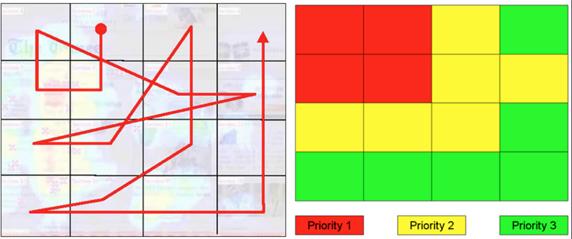
\includegraphics[width=\textwidth]{images/IlComportamentoDegliUtenti-FasceDAttenzione2}
				\caption[Il comportamento degli utenti - Movimento utente e zone calde pagina]{Il comportamento degli utenti - Movimento dell'utente e zone "calde" di una pagina}
				\label{fig:FasceDAttenzione2}
		\end{figure}
		
		\subsubsection{Fasce d'attenzione}
		
			Per misurare il movimento fatto da utenti in una pagina web si usa la tecnica dell'\emph{eyetracking} da cui si ricava una termografia di una pagina dove le zone calde corrispondono alle dove l'utente dedica più tempo mentre quelle più fredde quelle che non vede affatto se non nella prima fase di \emph{scanning}. Le diverse termografie classiche indicano che il \textbf{punto d'entrata} di una pagina web è \textbf{in alto a sinistra}. Le fasce d'attenzione risultano quindi avere una forma a \emph{F} o a \emph{cono gelato} come si può notare nella figura ~\ref{fig:FasceDAttenzione}.
			Nella maggioranza dei casi per ogni schermata della stessa pagina abbiamo una forma a \emph{F} nel punto in cui avviene lo \emph{scroll} si ha il \emph{blind spot} un punto cieco che non sarà mai visualizzato.
			
			\begin{figure} [h]
				\centering
				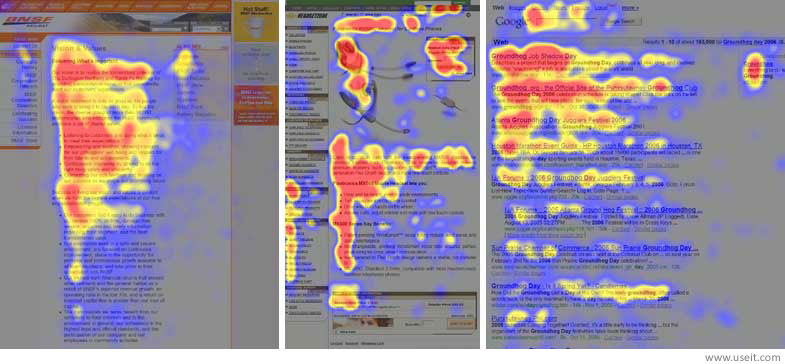
\includegraphics[trim={0 1pt 0 0}, width=\textwidth]{images/IlComportamentoDegliUtenti-FasceDAttenzione}
				\caption[Il comportamento degli utenti - Termografie]{Il comportamento degli utenti - Esempi di termografie}
				\label{fig:FasceDAttenzione}
			\end{figure}
		
		\subsubsection{L'importanza del testo}
			Al contrario dei giornali il testo è molto più rilevante rispetto alle immagini nel web. Per sfruttare questo ecco alcuni consigli per migliorare una pagina web.
			\begin{itemize}
				\item Il punto d'attrazione (in alto a sinistra) necessita di testo, il logo deve essere sempre accompagnato da qualche scritta magari che risponda all'asse What.
				\item Il testo su una singola colonna è meglio che su più colonne come nei giornali (l'effetto è molto simile alle liste \emph{itemize} orizzontali).
				\item Le \emph{keyword} messe vicine diluiscono l'importanza data nello \emph{scan}.
				\item Il \emph{bold} non basta per evidenziare le parole chiave. Meglio usare anche la sottolineatura (come un hyperlink) e ingrandire il \emph{font} o meglio ancora separare la o le \emph{keyword} in una riga a parte (una sorta di mini titolo).
			\end{itemize}
		
			\paragraph{Paragrafi e titoli}
				Un altro utile accorgimento per sfruttare l'importanza del testo è quello di dividere i grandi blocchi di testo in paragrafi corti (rispetto a quelli lunghi attraggono alla lettura quasi il doppio). Lo stesso possiamo dire dei titoli, più sono corti meglio è. Inoltre più un testo è spezzato in piccoli paragrafi più gli utenti sono incoraggiati a leggerlo rilassando i timer (suggerimento valido anche nelle mail).
				Sfruttare il \emph{blurp}, cioè aggiungere ad ogni titolo una mini descrizione per migliorare l'attrazione dell'intera pagina. I \emph{blurp} offrono vantaggi:
				\begin{itemize}
					\item rilassano i timer, ma non cambiano la voglia di proseguire nella navigazione del sito;
					\item aumentano il tasso di ritorno della pagina.
				\end{itemize}
				Il contenuto del \emph{blurp} non è un blocco unico ma può essere suddiviso in parti per cui ha una sua struttura e una sua termografia, per questo motivo le parole fondamentali devono stare alla sinistra del \emph{blurp}.
			
		\subsubsection{Pagine grasse o magre?}
			Per pagina grassa si intende una pagina web con contenuto più spaziato mentre con la pagina snella una pagina con contenuto più compatto. Dalle analisi è emerso che la pagina grassa funziona peggio. Bisogna infatti porre molta attenzione al separare il testo in paragrafi perché si può incorrere nel \emph{diluited design}. La spaziatura e la separazione portano ad uno \emph{scanning} più veloce ma ciò funziona male nelle pagine ricche di contenuto testuale. In generale:
			\begin{itemize}
				\item la \textbf{pagina grassa} è da preferire in quelle pagine di navigazione con link e poco \emph{scroll};
				\item la \textbf{pagina magra} invece è da preferire in quelle pagine con molto contenuto e tanto \emph{scroll}.
			\end{itemize}
		
		\subsubsection{Immagini nel web}
			Abbiamo visto che le immagini nel web hanno un ruolo marginale rispetto al testo difatti un'immagine affiancata ad un testo perde quasi tutta l'attenzione. Nonostante questo hanno comunque una proprietà (diversa dal testo) che le rende utili se sfruttata al meglio. Innanzitutto fissiamo una taglia minimi: 210x230 pixel, più piccola sembra un'icona e c'è rischio di ingannare l'utente. Le immagini hanno un tasso di click superiore al testo, solitamente il 20\% degli utenti clicca sull'immagine. Per sfruttare questo tutte le immagini dovrebbero essere cliccabili con evento correlato, l'utente è abituato cliccarci sopra e si aspetta sempre qualcosa.
			
			\paragraph{Slideshow}
				Ascoltiamo ora un esempio pratico di problemi all'interno del sito già citato varie volte \href{http://www.jcrew.com}{www.jcrew.com}.
				Lezione tenuta dal professor Marchiori: 
								
				\url{https://drive.google.com/open?id=0B3-HN4UsFMNfRHZWZDVRaWh0U1E} (minuto 39:50).
			
		\subsubsection{Lo spostamento dell'utente}	
			Se capiamo gli spostamenti dell'utente possiamo andargli incontro e incrementare la facilità d'uso del nostro layout con cui esso dovrà interagire. Fortunatamente una legge matematica viene in nostro soccorso.
		
			\paragraph{Legge di Fitts}
				Rappresenta il modello matematico del movimento umano in una singola dimensione (retta). La legge spiega quanto tempo impiega il cursore a spostarsi da un punto ad un altro.
			
					\begin{equation}
						\label{eqn:LeggeDiFitts}
						T=a+b \cdot \log_2 (1+\frac{D}{W})
					\end{equation}
					
					dove:
					\begin{itemize}
						\item $T$: è il tempo medio impiegato per concludere il movimento.
						\item $a$: tempo costante impiegato dall'essere umano per cominciare e concludere l'azione.
						\item $b$: covelocità, costante che dipende dagli strumenti utilizzati e dall'utente.
						\item $D$: distanza dal punto iniziale alla zona obiettivo.
						\item $W$: ampiezza della zona obiettivo.
					\end{itemize}
					Da notare che la distanza non conta molto nel tempo $T$ finale, ma pesa molto di più l'ampiezza del target finale $D$.
			
				\subparagraph{Past \& clink o drag \& drop?}
					Vediamo subito un esempio pratico della legge di Fitts ~\ref{eqn:LeggeDiFitts}. Meglio \emph{past \& click} o \emph{drag \& drop}? Applicando la legge di Fitts abbiamo che la covelocità per il \emph{drag \& drop} è maggiore a causa del muscolo in tensione, per cui \emph{past \& click} è da preferire nelle interfacce web.
			
				\subparagraph{Implicazioni della legge di Fitts}
					La principale implicazione che emerge è che gli \textbf{oggetti più grandi} sono \textbf{più facili} da raggiungere e cliccare. Ecco perché i menu sono odiati, non conta solo la distanza. I menu di navigazione devono essere più bilanciati. Altra implicazione è la \emph{target size rule}: la taglia di un pulsante dovrebbe essere proporzionale alla sua frequenza d'uso. Un ottimo esempio dell'uso della \emph{target size rule} è il redesign di Microsoft Office uscito nel 2007 (figura ~\ref{fig:ImplicazioniDellaLeggeDiFitts}.
					
					\begin{figure} [h]
						\centering
						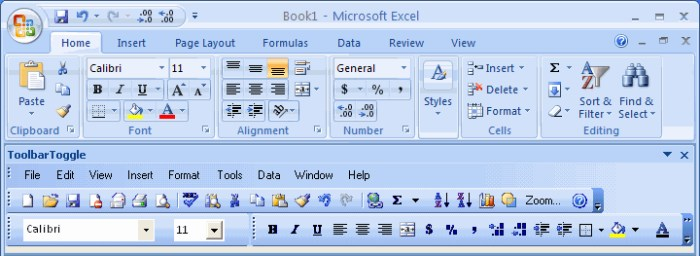
\includegraphics[width=\textwidth]{images/IlComportamentoDegliUtenti-ImplicazioniDellaLeggeDiFitts}
						\caption[Il comportamento degli utenti - Microsoft Office dopo e prima il restyling]{Il comportamento degli utenti - Microsoft Office dopo e prima il restyling}
						\label{fig:ImplicazioniDellaLeggeDiFitts}
					\end{figure}
				
				\subparagraph{Complicazioni}
					La legge di Fitts nasce considerando una dimensione, se l'area è uguale (variabile $W$) ma ha forma diversa? Quale pulsante è il migliore? Il pulsante migliore dipende dall'angolo creato dal punto di partenza e la retta. Per cui attenzione!
					
			\paragraph{Interfacce e Fitts}
				Altri esempi più fini dell'applicazione della legge di Fitts possiamo trovarli già dal primo sistema Macintosh. Il menu è fissato distante, in alto in modo da non avere problemi con l'asse y. Risultato: 5 volte più veloci in media dei menu Windows da qui poi nasceranno le \emph{task bar}. Ancora, lo strumento di \emph{scroll} su Mac ha una barra più lunga e i pulsanti sono vicini al contrario di Windows.
				
					\begin{figure} [h]
						\centering
						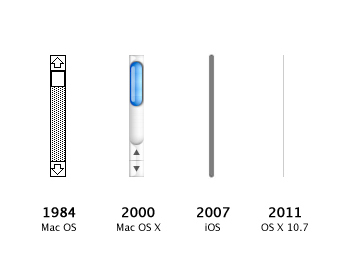
\includegraphics[scale=0.8]{images/IlComportamentoDegliUtenti-InterfacceEFitts}
						\caption[Il comportamento degli utenti - Evoluzione \emph{scrollbar} su Mac]{Il comportamento degli utenti - L'evoluzione della \emph{scrollbar} su Macintosh}
						\label{fig:InterfacceEFitts}
					\end{figure}
				
				\subparagraph{Zone magiche}
					Altri suggerimenti che nascono dalla legge di Fitts riguardano i bordi e ancora meglio gli angoli. Essi possono essere utilizzati come pulsanti d'interfaccia super efficaci perché non necessitano del tempo di frenata e l'area dell'obiettivo è molto grande a patto che l'utente non abbia una finestra ridotta sullo schermo. La figura ~\ref{fig:InterfacceEFitts} mostra esplicitamente come il sistema operativo Os X abbia sfruttato queste zone magiche per la \emph{scrollbar}. 
				
				\subparagraph{Menu 2.0}
					Anche nei menu possiamo vedere molti usi della legge di Fitts.
					\begin{description}
						\item[Menu a pop-up:] è un'estremizzazione di Fitts, abbiamo i pulsanti vicinissimi al cursore del mouse.
						\item[Menu circolare:] un evoluzione del \emph{menu a pop-up}, può esser completo (\emph{pie menu}) o solo in parte, da usare negli angoli soprattutto (\emph{fan menu}).
					\end{description}
					Tra i \emph{pie menu} e i \emph{menu lineari} non c'è dubbio che sull'usabilità vincono i primi, ma non sottovalutiamo i secondi che  per tanti elementi/comandi se combinati assieme ad altri tipi di menu possono dare risultati efficaci.
					Ricordiamo che i primi software ad implementare i menu 2.0 sono stati i videogame, l'uso del \emph{pie menu} in Second Life lo portò ad un gran successo. In altri l'uso dei pie menu permetteva di essere il più veloci possibili producendo eventi attraverso movimenti del mouse che aprivano catene di \emph{pie menu}.
				
				


\chapter{La pubblicità}
	Il modello di business classico è dare servizio gratis attraverso il web, ricevere utenti e sostenersi con la pubblicità. Piccolo intoppo: \textbf{gli utenti odiano la pubblicità}. Solo il 0,4\% clicca sulle pubblicità. Cosa fare per migliorare questa situazione e sopratutto far sì che l'utente clicchi su essa?
	\begin{itemize}
		\item Buon posizionamento banner.
		\item Messaggio efficace, bello e attraente.
	\end{itemize}

	\section{Posizionamento}
		Per quanto riguarda il posizionamento del o dei banner in coordinate assolute, per ordine di utilità, abbiamo:
		\begin{enumerate}
			\item Colonna di sinistra.
			\item Top della pagina.
			\item Colonna di destra.
			\item Bottom (non serve praticamente a nulla).
		\end{enumerate}
		Altri accorgimenti da adottare possono essere:
		\begin{itemize}
			\item Posizionare la pubblicità vicino al contenuto interessante così, maggiori visualizzazioni per essa.
			\item Rispettare le taglie minime e tener conto che la taglia non influenza molto. I banner grandi non attraggono molto di più di quelli piccoli.
		\end{itemize}
	
	\section{Messaggio efficace}
		Prima di analizzare come fare un messaggio pubblicitario efficace mostriamo le \textbf{11 cose} da \textbf{non fare} con percentuale di insoddisfazione generata agli utenti.
		
		\subsection{Top 11 disgrazie}
			\begin{etaremune}
				\item Suona automaticamente (79\%).
				\item È in movimento (79\%).
				\item Lampeggia (87\%).
				\item Occupa la maggior parte della pagina (90\%).
				\item Si sposta sullo schermo (92\%).
				\item Non dice di cosa si tratta (92\%).
				\item Copre il contenuto da leggere (93\%).
				\item Non dispone di un modo chiaro per chiudersi (93\%).
				\item È qualcosa che cerca di farti cliccare sopra (94\%).
				\item Si carica lentamente (94\%).
				\item È un pop-up (95\%).
			\end{etaremune}
		
		\subsection{Il mondo pubblicitario nel web}
			Per risaltare il messaggio nel mondo pubblicitario esistono accorgimenti molto efficaci come, ad esempio:
			\begin{itemize}
				\item Utilizzare persone belle per attirare l'attenzione.
				\item Usare colori vivaci ed effetti speciali.
			\end{itemize}
			Questi accorgimenti trasportanti nel web rimarranno efficaci?
		
			\subsubsection{Effetto zapping}
				Ricordiamo che le immagini nel web godono di meno visibilità e attenzione da parte dell'utente rispetto al testo, questo deriva da un processo automatico e subconscio (effetto \emph{zapping} nel web) che salta le immagini e soprattutto i banner. Portare infatti un contenuto in forma simile a immagini e banner può far sì che questo non sia nemmeno visualizzato dalla maggior parte degli utenti. 
				
				Gli utenti sono abituati a ritenere superflue le informazioni contenute nei banner per cui durante la navigazione il cervello utilizza dei filtri (che utilizziamo quotidianamente anche in altre situazioni) sull'informazione entrante dall'apparato visivo.		
			
		\subsection{Immagini in serie A}
			L'unico modo, paradossale, per rendere attrattive le nostre immagini e quindi banner è \textbf{andare controcorrente}. L'algoritmo abituale per filtrare è interrotto da qualcosa di inusuale e l'utente è costretto a porre maggiore attenzione. Quindi:
			\begin{itemize}
				\item Niente colori vistosi e attraenti.
				\item Confondere le idee all'utente.
			\end{itemize}
			Per far ciò si può ricorrere ad alcune tecniche:
			\begin{description}
				\item[Blending:] eliminare le zone della pubblicità confondendo pubblicità con contenuto. Il miglior \emph{blending} è il testo.
				\item[Giochetti web:] l'uso di giochi attira l'attenzione e azzera i timer dell'utente finché è impegnato a giocare. Una buona tecnica quindi è quella di inserire pubblicità insieme a giochi.
			\end{description}
			
			Attenzione però al \textbf{\emph{distraction effect}}: la pubblicità deve seguire il contesto in cui è contenuto altrimenti i timer dell'utente diminuiscono del 40\% e la voglia di rivisitare il sito scende addirittura dell'80\%.
		
		\subsection{Il problema del contenuto}
			Per risolvere il problema del contenuto e del \emph{distraction effect} si è ricorso al \emph{behavior advertising}, pubblicità che seguono il comportamento dell'utente nel web e che quindi è più probabile siano interessanti. Per far questo è necessario raccogliere dati su ogni singolo utente. Questo può rendere fino a 10000 volte più efficace la pubblicità e in certi casi ribalta l'insoddisfazione con aumento dei timer e voglia di ritornare al sito.


\chapter{La ricerca}
	Un altro problema fondamentale dei siti è far sì che il proprio contenuto sia trovato dagli utenti. La ricerca diviene quindi un fattore fondamentale all'interno del web. Esistono varie modalità di ricerca, prima di tutto ogni sito internet se abbastanza grande dovrebbe avere come servizio la ricerca interna e quindi vedremo come inserirla nel nostro sito garantendo l'usabilità ed discutendo problemi di molti siti. Scopriremo anche i motivi per cui diverse modalità di ricerca al primo impatto stupefacenti si rivelano essere fallimentari per l'usabilità dei siti internet, sono le ricerche 2.0 che con numerosi tentativi negli anni hanno cercato di sfruttare la sintesi vocale lottando contro il problema del contesto.

	\section{Ricerca interna}
		Una ricerca interna al proprio sito e la qualità di essa è determinata dal numero di pagine che questo ha.
		\begin{itemize}
			\item \textbf{>100} è \textbf{necessario} che il sito abbia uno strumento di ricerca.
			\item \textbf{>1000} è \textbf{cruciale} che lo strumento di ricerca sia eccellente e copra tutto il sito.
		\end{itemize}
		Si stima che la ricerca è utilizzata quasi nel 100\% dei casi. Gli utenti sono abituati ai motori di ricerca e molto spesso gli utenti arrivano in una pagina qualunque del sito attraverso il \emph{deep linking}. Difatti:
		\begin{itemize}
			\item il 60\% usa la ricerca appena giunge in un sito (se essa è disponibile).
			\item il 40\% fa uso di link.
		\end{itemize}
		
		Vista l'enorme importanza in molti siti si tende ad inserire uno strumento di ricerca, ma questo se fatto come si deve è molto costoso e troppo spesso si incorre all'uso di soluzioni \emph{low cost} che peggiorano soltanto la situazione. Solitamente questa soluzione è di localizzare motori di ricerca sul proprio sito, il costo è nullo ma:
		\begin{itemize}
			\item l'algoritmo dei motori di ricerca è ottimizzato per larghe scale, su bassa scala non dà risultati soddisfacenti.
			\item Se l'utente usa la ricerca significa molto probabilmente che il motore di ricerca già utilizzato non l'ha portato al suo scopo per cui utilizzarlo ancora non servirà a niente.
			\item I motori di ricerca non fanno la lettura di tutte le pagine (il 70\% del web è sconosciuto ai motori di ricerca) per cui questo può far sì che alcune pagine del sito non compariranno mai tra i risultati.
		\end{itemize}			
	
		\subsection{Ricerca su misura}	
			Gli utenti preferiscono:
			\begin{itemize}
				\item 1 sola modalità di ricerca come i motori di ricerca.
				\item Un \textbf{box testuale} e un \textbf{pulsante} con scritto "search" (o "cerca"). Null'altro è da sostituire alla parola "search".
				\item Si può sostituire il box testuale e il pulsante con l'icona della lente per siti mobile. In generale però gli utenti preferiscono sempre il testo.
			\end{itemize}
	
			\subsubsection{Principio di Robert Browning}
				Enunciamo un principio che nel web ha praticamente valenza generale. Il primo ad annunciarlo fu Robert Browning e in seguito fu ripreso dall'architetto modernista Ludwig Mies van der Rohe.
				\begin{quote}
					``\emph{Less is more}''
				\end{quote}
				Che applicato al web consiste in: \emph{``meno dettagli e orpelli significa qualcosa di meglio''} (cit.). L'esempio lampante è la pagina iniziale del motore di ricerca Google.
				Ludwig Mies van der Rohe estese anche il principio in:
				\begin{quote}
					``\emph{Less is more but God is in the detail}''
				\end{quote} 
				Per capire quanto i dettagli sono importanti si veda l'Errore 404 ~\ref{sec:error404}.
	
	\section{Ricerca vincolata}
		La ricerca vincolata si prefigge di accompagnare l'utente passo passo attraverso parametri, deve essere considerata come un'aggiunta alla classica ricerca spiegata in precedenza. Vantaggi e svantaggi:
		\begin{itemize}
			\item è efficiente e gradita dagli utenti.
			\item esistono due modalità di come si offre ognuna con i suoi svantaggi.
		\end{itemize}
		
					
		\subsection{Ricerca vincolata dinamica}
			La ricerca dinamica avviene per ogni settaggio di parametro.
			Svantaggi:
			\begin{itemize}
				\item Quando il numero dei vincoli è grande l'attesa del caricamento è alto.
				\item Abbiamo un carico del server notevolmente maggiore.
				\item Se l'utente ha già i vincoli in mente dovrà fare comunque più ricerche.
			\end{itemize}
	
		\subsection{Ricerca vincolata statica}
			La ricerca avviene solo nel momento in cui l'utente ha impostato tutti i parametri richiesti e ha dato il via.
			Svantaggi:
			\begin{itemize}
				\item Il pulsante non ha contenuto standard. Le parole "search" o "cerca" illudono che sia la ricerca classica. 
				\item Se un utente è abituato a quella dinamica resta confuso al prima impostazione di parametro perché non succede nulla. Questo può indurlo a pensare che non funzioni.
			\end{itemize}
		
		\subsection{Soluzione ibrida}
			In generale la soluzione dinamica è meglio nel caso in cui un utente non sappia cosa cercare mentre è il contrario per la ricerca statica. Esiste una terza soluzione (ibrida) che consiste nell'avviare la ricerca automaticamente al termine del settaggio dei parametri. In questo modo togliamo il pulsante per la ricerca statica e non appesantiamo il server con ricerche superflue.
		
	\section{Consigli}
		Di seguito elenchiamo alcuni consigli per mostrare i risultati di ricerca nel migliore dei modi.
		\begin{description}
			\item[Ordinamento:] mettere sempre a disposizione un ordinamento bidirezionale.
			\item[Casi limite:] se non ci sono risultati dobbiamo comunicare all'utente che ci non ci sono risultati, altrimenti si confonde l'utente che pensa non funzioni.
			\item[Error 404:] \label{sec:error404} quando i link sono "rotti" (non esistono più) deve esserci una pagina con suggerimenti all'utente che offrono aiuto. Molte volte a queste si affianca qualcosa di simpatico che ironizza la situazione, ciò sospende i timer, un esempio di questo lo troviamo nella pagina 404 del sito \href{http://www.b3ta.com/error404}{www.b3ta.com}, che raccoglie le più esilaranti immagini delle pagine error 404 nel web.
			\item[Presentazione risultati:] esistono due modi per presentare i risultati di una ricerca.
				\begin{itemize}
					\item Modalità classica: vedi figura ~\ref{fig:LaRicerca-Consigli}.
					\item Modalità a griglia: permette di visualizzare molta più informazione compatta ma questo fa sì che gli elementi mostrati perdano rilevanza. Con questa modalità l'utente si confonde e si perde nella micro-navigazione. Non a caso Google immagini propone i risultati a griglia, vuole che l'utente stia per più tempo all'interno del sul motore di ricerca. (vedi figura ~\ref{fig:LaRicerca-Consigli})
				\end{itemize}
		\end{description}
		
		\begin{figure}
			\centering
			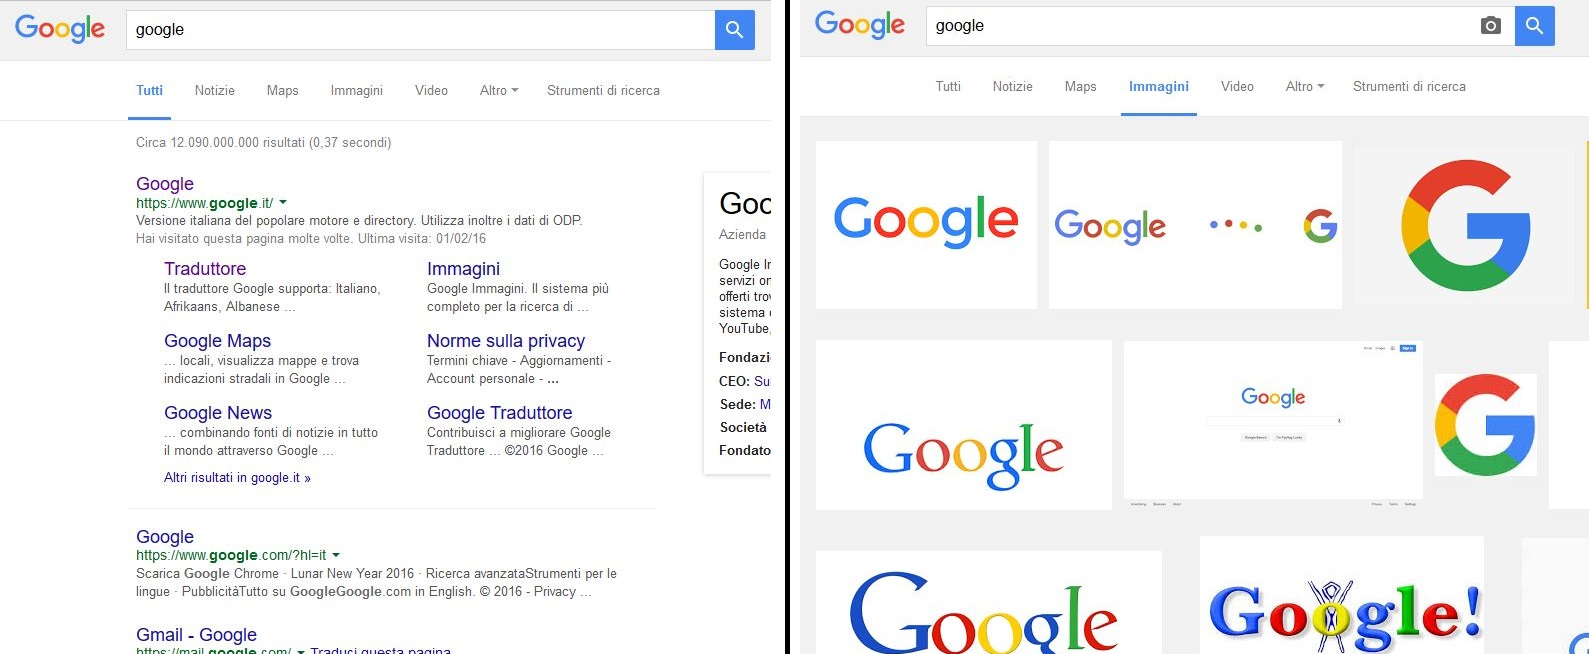
\includegraphics[width=\textwidth]{images/LaRicerca-Consigli}
			\caption[La ricerca - Tipi di presentazioni risultati]{La ricerca - Presentazione dei risultati lineare e a griglia}
			\label{fig:LaRicerca-Consigli}
		\end{figure}
		
	\section{Il search box}
		Agli arbori del web nelle caselle di ricerca si inserivano nella maggior parte dei casi parole uniche, con il passare del tempo però gli utenti usano sempre più parole. Il numero massimo di caratteri determina il numero di utenti a cui basterà.
		\begin{itemize}
			\item con 10 caratteri solo il 35\% degli utenti sarà soddisfatto.
			\item con 30 caratteri l'88\%.
		\end{itemize}
		Quest'ultimo numero è la media consigliata. Un box troppo piccolo aumenta lo stress proporzionalmente per ogni carattere che sfora e gli utenti tendono a scrivere meno con risultati della \emph{query} più scarsi.
		Per la necessità di spazio per il design in molti casi si è ricorso ad un \textbf{box dinamico} che una volta cliccato si allarga per contenere più caratteri.
	
	\section{Ricerce 2.0 (*)}
		(N.B. la seguente sezione è incompleta)
		
		Il web è un media informativo visivo. Negli anni sono stati vari i tentativi di evolvere dal testo alla voce per un'interazione uomo-macchina di livello superiore. Esistono varie tecnologie:
		\begin{itemize}
			\item VoiceXML
			\item SSML
			\item PLS
			\item CCXML
			\item SRGS
		\end{itemize}
		che via via hanno migliorato l'interazione uomo macchina ma si è ancora lontani da \emph{HALL 9000} il supercomputer intelligente di \emph{2001: Odissea nello spazio}.
		
		\subsection{Il grande problema}
			Basarsi sulla voce non basta perché rende difficile interpretare le parole senza l'aiuto del \textbf{contesto}.
			La tecnologia \emph{Google Glass} non ha avuto successo proprio per questo motivo, l'utenza chiedeva più pulsanti perché la sintesi vocale non era sufficiente.
			
		\subsection{L'utente e le ricerche 2.0}
			Le ricerche del 2.0 diminuiscono la soddisfazione del 42\%! Perché?
			\begin{itemize}
				\item Di fronte ad un assistente virtuale l'utente si forma aspettative più alte e per questo diventa ancora più esigente.
				\item Illudere l'utente presentando un robot simile all'umano non aiuta, molto meglio mantenere un'interfaccia robotica per non dare illusioni e creare grosse aspettative.
			\end{itemize}
			Un esempio positivo che segue questi accorgimenti è \emph{Anna} di IKEA. Vediamone i punti forti:
			\begin{itemize}
				\item riceve in input solo testo e presenta un \emph{engine} linguistico ben fatto. 
				\item Ha un'interfaccia \emph{cartoon}.
				\item È uno strumento facoltativo.
			\end{itemize}
		
		\subsection{Involuzione/evoluzione dell'interazione}
			Per il problema del contesto nei videogiochi si è sempre più limitata la libertà di scelta e interazione negli anni. Ciò perché un grado di libertà alto poteva generare incomprensioni tra utente e macchina e la frustrazione aumentava.
		
			\subsubsection{Il rumore}
				Un altro motivo per cui le interfacce non precise hanno un gradimento superiore è il rumore di fondo. È grazie al rumore di fondo che sembrano più naturali. A tal proposito si sono fatti studi sul rumore che costantemente viviamo. Esso ha una natura frattale ricorsiva e per generarlo basta continuare a \textbf{ridurre l'ampiezza} e \textbf{alzare la frequenza} e infine mettere insieme tutte le parti.
				Paradossalmente le interfacce imperfette danno più soddisfazione.


\chapter{La visibilità}

Altra caratteristica essenziale per l'informazione all'interno di un sito è l'essere trovata. Per far ciò conta la \textbf{visibilità esterna} e questa è determinata dal posizionamento del sito sui motori di ricerca. 
	Vedremo che è essenziale posizionarsi nella top 10 per le \emph{keyword} che ci riguardano e capiremo come promuovere un sito analizzando il funzionamento dei \emph{search engine} (SE) e l'uso che gli utenti ne fanno.

	\section{Posizionamento SERP}	
		La top 10 risultati assorbe il 95\% dei click dell'utenza dopo una ricerca.
		\begin{enumerate}
			\item 51\% click (il primo risultato prende più di tutte le altre!),
			\item 16\% click;
			\item 6\% click;
			\item 6\% click;
			\item 5\% click;
			\item 4\% click;
			\item 2\% click;
			\item 1\% click;
			\item 1\% click;
			\item 2\% click (effetto \emph{black jersay} o \emph{Malabrocca}).		
		\end{enumerate}
		
		Nota: le strategie che verranno illustrate in seguito non funzionano sempre, basta infatti un minimo cambiamento per cambiare il comportamento degli utenti sui risultati. Infatti recenti introduzioni di Google sono state analizzate molto, prima di farle diventare effettive. La striscia di immagini per esempio svolgono un effetto sospensivo per trattenere l'utente e non hanno impatto sulla percezione del testo.
	
	\section{SPAMDEX (SEO)}
		È l'insieme di attività svolte con lo scopo di far sì che un sito sia indicizzato da Google e occupi le posizioni più alte della SERP. Nelle seguenti sezioni prima spiegheremo il funzionamento dei motori di ricerca e poi illustreremo le tecniche per migliorare il posizionamento o addirittura ingannare il SE.
		Il \textbf{punteggio di una pagina} è calcolato sul riferimento a due componenti delle pagine:
		\begin{itemize}
			\item componente \textbf{testuale};
			\item componente \textbf{ipertestuale}.
		\end{itemize}
		
		\subsection{Parte testuale}
			Per la parte testuale si misura la qualità in base a quanto una parola è importante per una pagina attraverso il TFIDF. Per misurare l'importanza di una parola si utilizzano due tecniche:
			
			\subsubsection{Term frequency (TF)}
				Misurare la frequenza di una parola. Ad esempio su 100 parole in una pagina 5 sono di nostro interesse per cui il TF è uguale al 5\%.
				È ovvio che solo questa tecnica non basta per avere risultati soddisfacenti, parole molto frequenti come articoli, congiunzioni, eccetera avrebbero un'importanza troppo alta anche se prive di significato.
				
			\subsubsection{Inverse document frequency}
				È la misura dell'inverso della frequenza della parola nell'insieme dei documenti (il sito web) scalata logaritmicamente. 
				
				Esempio: su 1000 pagine "il" appare in 980 pagine, ha TF=98\% mentre:
				\[
					IDF=\log \left(\frac{1}{0,98} \right)=0,008;
				\]
				
				Altro esempio: su 1000 pagine la parola "pippo" ha il 10\% di frequenza, allora:
				\[
				IDF=\log \left(\frac{1}{0,1} \right)=1;
				\]
				
				Ora più rara è la parola più è alto il bonus.
				
			\subsubsection{Query SE}
				Ogni \emph{query} sarà composta dalle parole con cui il SE andrà a calcolare TF e IDF nei siti web. Quelli con il valore più alto si posizioneranno più in alto.
				Se sottoponiamo una \emph{query} con una parola $p$  il SE prende le pagine dove appare $p$ e ne calcola il TF e l'IDF. Per più parole in una \emph{query} si usa la somma del TF e IDF.
				In questo modo alzare il punteggio di una parola può rischiare di diluire il valore e viceversa. È importante quindi selezionare un gruppo di parole e alzare il loro TFIDF a scapito di altre, queste \emph{keyword} saranno le parole che competeranno nella SERP.
			
		\subsection{Term spam}
			Vediamo quindi alcune tecniche per aumentare il punteggio per le \emph{keyword} definite.
			\begin{description}
				\item[Body spam:] inserire le \emph{keyword} semplicemente nel body html.
				\item[Title spam:] inserire le \emph{keyword} sul titolo delle pagine web, è una parte che l'utenza media non vedrà mai.
				\item[Meta tag spam:] inserire le \emph{keyword} in appositi tag html (i \emph{meta}) che descrivono a \emph{keyword} la pagina. Per l'inteso sfruttamento i SE oramai ignorano questo genere di spam.
				\item[Anchor text spam:] inserire le \emph{keyword} nel testo di un link tra i tag \verb|<a>...</a>|. Questo oltre al punteggio della pagina aumenta il punteggio alla pagina destinazione e il bonus viene dato con meno limiti per il TFIDF.
				\item[URL spam:] inserire le \emph{keyword} nell'URL dell'indirizzo della pagina. Otteniamo bonus simili a quelli dell'\emph{anchor text spam}.
			\end{description}
			
		
			\subsubsection{Starter kit}
				Abbiamo visto dove inserire le \emph{keyword}. Ora vediamo le tecniche utilizzate di come inserirle:
				\begin{description}
					\item[Repetition:] ripetere la \emph{keyword} stando attenti al suo TFIDF. Tecnica facile da trovare dal SE che può pure penalizzare.
					\item[Dumping:] inserire termini rari nel testo anche se non c'entrano nulla. Otteremo un punteggio alto sul sito anche se questo non è pertinente.
					\item[Wearing:] utilizzare pezzi di altre pagine web in cui sono inserite le nostre \emph{keyword} in modo random.
					\item[Stitching:] \emph{past \& copy} da siti differrenti e si assembla il tutto ottenendo un contenuto rilevante. Per esempio da una risposta di un utente su un forum sviluppiamo un articolo nuovo. Più argomenti diversi danno inoltre un bonus globale e i SE fanno fatica a capire se è contenuto copiato.
					\item[Broeding:] oltre alle \emph{keyword} fare uso di sinonimi e frasi correlate. Questo coprirà più le \emph{query} degli utenti.
				\end{description}		
		
			\subsubsection{Quali keyword?}
				Una domanda di cui la risposta probabilmente decreterà il successo di un sito. Le \emph{keyword} devono essere pensate in base a quello che cerca l'utente. Occorre un'attenta analisi prima di lanciarsi nel mondo SEO. Di seguito alcuni strumenti utili a tale scopo:
				\begin{itemize}
					\item \href{https://adwords.google.com/KeywordPlanner}{Google keyword tool} (a pagamento);
					\item \href{http://keywordtool.io/}{keywordtool.io} (alternativa gratis);
					\item \href{https://www.google.it/trends/}{Google Trends} (ottimo per capire la tendenza nel tempo);
				\end{itemize}
			
		\subsection{Problema e soluzioni del term spamming}
			Non basta potenziare la pagina, se infatti questa non è utile e soffre di problemi di usabilità l'utente semplicemente abbandonerà. Se vogliamo potenziare una pagina con le tecniche di \emph{term spamming} dobbiamo nascondere in qualche modo all'utente ciò che serve ai SE.
		
			\subsubsection{Content hiding}
				Il contenuto potenziante è nascosto all'utente e solo i motori di ricerca lo vedono.
			
			\subsubsection{Redirection}
				Anche detta tecnica 302, consiste nel potenziare una pagina che sarà costruita con soli fini di posizionamento che indirizza alla vera pagina. In questo modo gli utenti vedranno la pagina studiata per loro mentre i SE si fermeranno a leggere la prima. Questa tecnica funziona solo con trucchetti che richiedono \emph{javascript}, il \emph{meta} che reindirizza infatti è riconosciuto dai SE. Con l'uso di \emph{javascript} il \emph{meta} verrà aggiunto dinamicamente e i SE, per costi di risorse, non si accorgeranno poiché non eseguono il codice. Tuttavia ad oggi i SE leggono il codice \emph{javascript} e cercano se esiste questa tecnica, per ingannarli è sufficiente offuscare un po' il codice.
			
			\subsubsection{Cloaking}
				Controlla l'accesso alla pagina per capire se chi visita è un bot o un umano. Se questo è un bot li presento una pagina apposita diversa da quella mostrata all'utente. È una tecnica difficile da scoprire tanto che Google la penalizza moltissimo se segnalata ma questo avviene solo tramite intervento umano.
			
	
		\subsection{Parte ipertestuale: pagerank}
			Il punteggio delle pagine web è affidato anche ai link di ipertesto: il \emph{pagerank}. Ad ogni pagina $\pi_v$ era affidato un punteggio pari a:
				\[
					\pi_v=\sum_{(\omega, v) \in E}\frac{\pi_{\omega}}{d_w}
				\]
			Dove:
			\begin{itemize}
				\item $\omega$, $v$ è un link da $\omega$ a $v$;
				\item $d_\omega$ è il numero di link uscenti.
			\end{itemize}
			Ossia, se una pagina $\omega$ ha un link verso un'altra pagina viene data una frazione ($1/d_\omega$) di \emph{pagerank} a quest'ultima.
			Come vincolo abbiamo:
			\[
				\sum\pi_v=1
			\]
			
			Questo calcolo di \emph{pagerank} molto naive era molto facile da manipolare con gli stratagemmi visti in precedenza, si è deciso quindi di farne una riformulazione.
		
			\subsubsection{Le catene di Markov e il random walk}
				La riformulazione avviene sfruttando l'algebra lineare e speciali matrici dette catene di Markov che godono di alcune proprietà unite alla teoria della probabilità. Il \emph{pagerank} di una pagina web diventa quindi la probabilità di entrare in quella pagina da altre pagine.
				Per rendere più chiaro il concetto si può pensare ad una scimmia  (un \emph{random surfer}) che naviga il web in modo del tutto casuale, la probabilità che la scimmia entri in una pagina ne determina il suo punteggio.
				
				Esempio:
					dato il seguente grafo i nodi che rappresentano pagine e gli archi i link:
					$A \longleftrightarrow B \longleftrightarrow C$,
					
					B ottiene il 50\% del flusso mentre A e C il 25\%.
					
				Il \emph{random surfer} è un altro fattore su cui tener conto ma attenzione esso non rispecchia esattamente gli intenti degli utenti che non navigano totalmente a caso.
			
			\subsubsection{Problemi: spider traps e island}
				Per attuare il sistema spiegato in precedenza c'è la necessità di far girovagare questi \emph{random surfer} (i famosi \emph{spider}) che raccolgono dati da cui calcolare il \emph{pagerank}. La navigazione casuale da pagina a pagina può rivelarsi fatale in alcuni casi.
				\begin{description}
					\item[Spider traps:] nel caso in cui uno spider rimanga intrappolato all'interno di un sito in cui pagine continuano a indirizzare ad altre pagine in un ciclo infinito (si pensi ad un calendario online).
					\item[Island:] esistono poi casi in cui alcuni pezzi di rete sono isolati dagli altri, dei veri e propri micro-web indipendenti in cui per gli \emph{spider} non c'è alcun modo di passare, ciò significa: nessun valore di \emph{pagerank} o infiniti valori diversi di \emph{pagerank}.
				\end{description}
				
		\subsection{Pagerank 2.0}
			A seguito dei problemi prima elencati si è cercato un'altra soluzione: il teletrasporto. La formula quindi cambia in (con $N$ numero totale di pagine):
			\[
				\pi_v=(1-\epsilon)\cdot \left( \sum_{\omega, v \in E} \frac{\pi_{\omega}}{d_w} \right) + \frac{\epsilon}{N}
			\]
			Nella pratica si è aumentata la casualità. Ora la scimmia ha anche un dado,  con una certa probabilità effettua il teletrasporto in un'altra pagina casuale altrimenti fa come spiegato in precedenza (da notare un comportamento apparentemente più strano se paragonato con quello degli utenti, in realtà non poi così tanto poiché molte volte un utente effettua il teletrasporto attraverso URL diretto).
			
			In questo modo grazie al \textbf{fattore di teleporting} $\epsilon$ risolviamo \emph{spider traps} e \emph{island}; più questo fattore è verso il 100\% e più il punteggio in probabilità alle pagine diventa uguale per tutte, viceversa più è verso lo 0 e più il \emph{pagerank} si avvicina a quello calcolato in precedenza.
			
			Un altro modo per il calcolo del \emph{pagerank} è il \emph{total rank}:
			\[
				T=\int_0^1r(\alpha) d\alpha
			\]
			
		
			\subsubsection{Problema: dead ends}
				Nonostante l'introduzione del teletrasporto rimane il problema (prima non illustrato) delle \emph{dead ends}. Con questa formula l'egoismo paga, un sito è meglio che mantenga i link al suo interno.
				
				La soluzione a cui sono arrivati i moderni motori di ricerca è calcolare l'importanza su altro per ogni sito e pagina web e non sul vero web. (vedere paragrafo ~\ref{sec:email})
		
		\subsection{Migliorare il pagerank}
			Esistono due fattori fondamentali che influenzano il \emph{pagerank} con l'uso del teletrasporto:
			\begin{itemize}
				\item Inlink;
				\item Outlink.
			\end{itemize}
		
			\subsubsection{Inlink}
				Link entranti alla pagina. Per incrementare il \emph{pagerank} di una pagina dobbiamo fare in modo che questa sia puntata dal maggior numero di pagine esterne. Alcune tecniche per fare ciò sono:
				\begin{description}
					\item[Infiltration:] infiltrarsi in altri siti e mettere link alla pagina da potenziare (commenti spam etc.).
					\item[Honey pot:] creare contenuto appetibile e utile che riceve link (è il modo giusto di aumentare il \emph{pagerank}). Molto spesso questo contenuto è vittima del \emph{copy \& past}.
					\item[Link exchange:] allearsi con altri per scambiarsi link.
					\item[Resurrection:] acquistare domini defunti con \emph{pagerank} abbastanza alto. Il \emph{pagerank} infatti non decade mai e resta legato al dominio, inoltre l'età del dominio conta come bonus. Esistono interi business per la vendita di domini defunti ma appetibili per il proprio \emph{pagerank}.
				\end{description}
				
				\paragraph{Marketing 2.0}
					Un esempio nella storia del web di quanto siano importanti gli \emph{inlink} arriva dalla pagina \href{http://www.milliondollarhomepage.com/}{million dollar page}. Una schermata di pixel venduta a 1 dollaro l'uno, il punto forte per cui tutti si affrettarono di acquistare almeno 1 pixel fu la presenza di tutti i link che puntavano alla pagina resa famosa dall'originale idea dell'autore. La pagina diventò una vera e propria cascata di flusso per il \emph{pagerank} ed ogni link al suo interno ne acquistava un po' ad un prezzo ridicolo.
			
			\subsubsection{Outlink}
				Passiamo ora ai link uscenti. Posizionando un link esterno in una pagina un po' di flusso di \emph{pagerank} esce dalla pagina. In questo modo è garantita la \textbf{solidità}, l'aggiunta di \emph{outlink} non alza il punteggio e lo \emph{smapdex} non può essere locale.
				Questo controintuitivamente non risulta essere vero! Con la presenza di \emph{outlink} posso aumentare il \emph{pagerank} della mia pagina con dinamiche imprevedibili. Ciò deriva dalla presenza del \emph{fattore di teleporting}.
			
			\subsubsection{Spam farm}
				Esistono numerose tecniche per usare gli \emph{outlink} e gli \emph{inlink} per aumentare il \emph{pagerank}. Le \emph{spam farm} sono una di queste tecniche: strutture apposite studiate di link e pagine per l'incremento del punteggio nei vari SE. 
				Una \emph{spam farm} ottimale singola consiste in una pagina o più pagine, definite pagine \textbf{target}, puntate da link bidirezionali da altre pagine, definite pagine \textbf{potenzianti}. Un struttura ottimale inoltre presenta la proprietà di \emph{reachability}, ovvero se gli spider dei SE raggiungono la pagina \emph{target} attraverso una pagina \emph{potenziante} allora tutta la \emph{spam farm} diventa raggiungibile (vedere figura ~\ref{fig:LaVisibilita-SpamFarm1}).
				
				\begin{figure} [h]
					\centering
					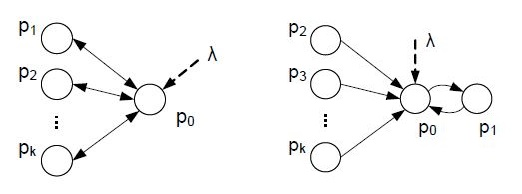
\includegraphics[scale=0.9]{images/LaVisibilita-SpamFarm1}
					\caption{La visibilità - Esempi spam farm singole ottimali}
					\label{fig:LaVisibilita-SpamFarm1}
				\end{figure}
				
				\paragraph{Alleanze}
					Il modo migliore per sfruttare le \emph{spam farm} è sfruttare alleanze con altri siti internet. Le alleanze tra siti (due e più) possono essere di tipo:
					\subparagraph{Alleanza profonda}
						Le pagine target distribuiscono il flusso sulle pagine potenzianti dell'altro sito (figura ~\ref{fig:LaVisibilita-SpamFarm2}) creando una media dei \emph{pagerank} stabile.
						
					\begin{figure} [h]
						\centering
						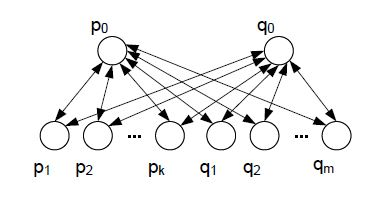
\includegraphics[scale=0.9]{images/LaVisibilita-SpamFarm2}
						\caption{La visibilità - Spam farm alleanza profonda}
						\label{fig:LaVisibilita-SpamFarm2}
					\end{figure}
						
					\subparagraph{Alleanza superficiale}
						Le pagine target dei due siti sono connesse con link (figura ~\ref{fig:LaVisibilita-SpamFarm3}, il \emph{pagerank} ottenuto risulta essere più del massimo delle due pagine target prima della connessione.
					
				\begin{figure} [h]
					\centering
					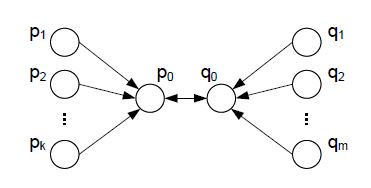
\includegraphics[scale=1]{images/LaVisibilita-SpamFarm3}
					\caption{La visibilità - Spam farm alleanza superficiale}
					\label{fig:LaVisibilita-SpamFarm3}
				\end{figure}
				
					\subparagraph{Alleanze Ring}
						Alleanza che comprende più di due siti. Le pagine target indicizzano in un percorso circolare la pagina target successiva creando una sorta di anello (figura ~\ref{fig:LaVisibilita-SpamFarm4}).
						
				\begin{figure} [h]
					\centering
					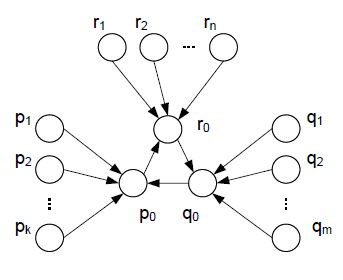
\includegraphics[scale=1]{images/LaVisibilita-SpamFarm4}
					\caption{La visibilità - Spam farm alleanza ring}
					\label{fig:LaVisibilita-SpamFarm4}
				\end{figure}
				
					\subparagraph{Alleanza complete core}
						Potenziamento della \emph{spam farm} di tipo \emph{ring}, la struttura bidirezionale è più vantaggiosa. Ora ogni pagina target ha link entrante e uscenti verso le due pagine target più vicine (figura ~\ref{fig:LaVisibilita-SpamFarm5}). Per fare un core basta un grafo fortemente connesso.
				
				\begin{figure} [h]
					\centering
					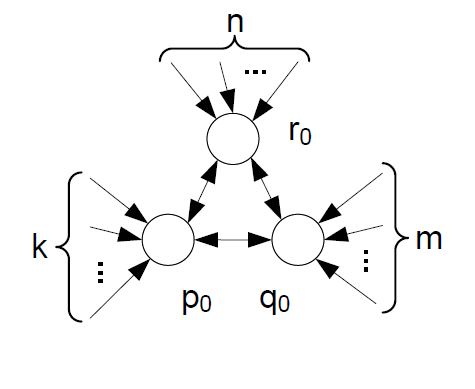
\includegraphics[scale=0.6]{images/LaVisibilita-SpamFarm5}
					\caption{La visibilità - Spam farm alleanza complete core}
					\label{fig:LaVisibilita-SpamFarm5}
				\end{figure}
				
			\subsubsection{Contromisure SE}
				Ovviamente le \emph{spam farm} sono azioni penalizzate dai SE poiché ingannano la misura del \emph{pagerank}. I motori di ricerca controbattono quindi cercando di identificare queste unioni rivelando l'esistenza di grafi fortemente connessi. Questi grafi dipendono dal modo con cui l'alleanza si è creata e dal numero di partecipanti ad asse. Visto il numero enorme di combinazioni fu creata un'enciclopedia delle sequenze. Purtroppo in ogni sequenza il numero di collegamenti da controllare cresce enormemente in base al numero di partecipanti (N), per:
				\begin{itemize}
					\item N=3 $\rightarrow$ 18 collegamenti;
					\item N=4 $\rightarrow$ 1606 collegamenti;
					\item N=5 $\rightarrow$ 565080 collegamenti;
					\item \dots
				\end{itemize}
				Non esiste nessuna formula che calcoli il risultato di collegamenti dato un numero N di partecipanti. Inoltre il costo computazionale risulta dispendiosissimo. Si sono quindi cercate soluzioni "laterali" più sofisticate.
				
				Un modo consiste in calcolare il vecchio \emph{pagerank} e confrontarlo con quello nuovo. Se il rapporto tra le due misure risulta troppo alto significa che la pagina analizzata è potenziata. È stato stimato che il successo di questa tecnica si trova tra il 95\% e 100\%.				
				
				Un altro modo consiste nel basarsi sulla \textbf{forma del web}: la struttura di alto livello a papillon (figura ~\ref{fig:LaVisibilita-FormaWeb}). L'idea è di analizzare la forma di un sito web, se questa non rispecchia ed ha valori al di fuori della media nella norma globale dei siti web allora il sito è sospetto e avviene un controllo più approfondito.
				Nella figura ~\ref{fig:LaVisibilita-ContromisureSE1} vediamo la zona creata dai link entranti nei siti nel web globale che rappresenta la norma. I punti situati all'esterno (evidenziati dall'ellisse) sono siti di cui si sospetta il potenziamento. Nella figura ~\ref{fig:LaVisibilita-ContromisureSE2} invece vediamo i link uscenti. 
				
				\begin{figure}
					\centering
					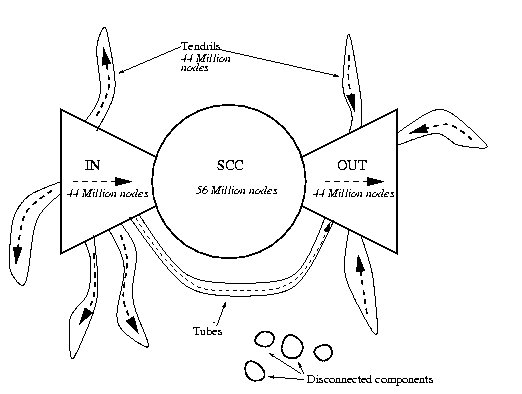
\includegraphics[scale=0.6]{images/LaVisibilita-FormaWeb}
					\caption{La visibilità - Forma ad alto livello del web}
					\label{fig:LaVisibilita-FormaWeb}
				\end{figure}								
				
				\begin{figure} [h]
					\subfloat[][\emph{Distribuzione link entranti}.]
						{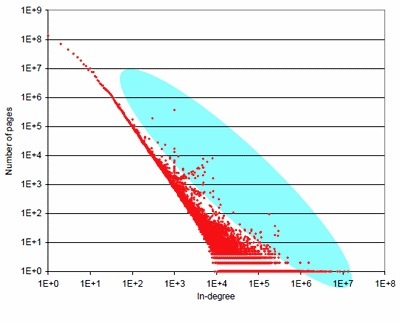
\includegraphics[width=.48\textwidth]{images/LaVisibilita-ContromisureSE1}
						\label{fig:LaVisibilita-ContromisureSE1}} \quad
					\subfloat[][\emph{Distribuzione link uscenti}.]
						{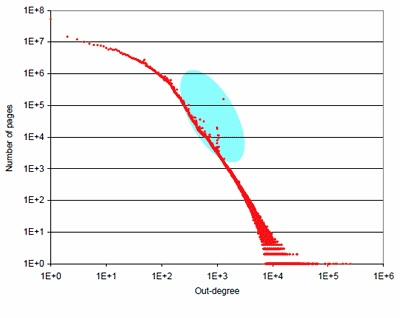
\includegraphics[width=.48\textwidth]{images/LaVisibilita-ContromisureSE2}
						\label{fig:LaVisibilita-ContromisureSE2}}
					\caption{La visibilità - Rappresentazioni grafiche dei link nel web}
					
				\end{figure}
			
		\subsection{Pagerank 3.0}
			Negli ultimi anni si è voluto migliorare la formula del \emph{pagerank} in particolare il fattore di teleporting.
			
			La vecchia formula (qui riporta in una versione leggermente diversa):
			\[
				(1-\epsilon )\cdot 1^T N + \epsilon L
			\]
			possiamo scriverla usando la matrice $P$ e diventa:
			\[
				(1- \epsilon )\cdot 1^T N + PL
			\]
			$P$ è una matrice che permette il \emph{pagerank} personalizzato che sostituisce il teletrasporto. Ogni nodo è pesato con preferenze così rendiamo il teletrasporto meno stupido. In questo modo però sorgono problemi riguardanti la libertà e la censura. Se infatti l'utente delle preferenze è il SE di turno, potrebbe volutamente alzare il \emph{pagerank} ad alcuni siti e abbassarlo ad altri. 
			
			È noto che Google personalizza la bontà di un sito, alcune sono addirittura fatte a mano! \emph{Searchking}, competitor di Google, è stato penalizzato in questo modo e il ricorso legale ha rivelato come il \emph{pagerank} sia soltanto un'opinione.
			Con questo nuovo livello di \emph{pagerank} quindi possiamo dichiarare defunta la democrazia contenuta in esso.
		
			\subsubsection{Pagerank personalizzato}
			
				Il \emph{pagerank} personalizzato però non è disponibile soltanto ai SE ma anche all'utente. Ogni profilo personale di ogni utente calcola un \emph{pagerank} personalizzato in base a tutti i dati raccolti su di lui (vedi tutte le piattaforme Google disponibili che ogni giorno utilizziamo tutti).  In questo modo i risultati di ricerca varieranno in base ai suoi interessi.
				Ma come calcolare questo \emph{pagerank} personalizzato per ogni utente nel web!? Se restringiamo a soli due valori: "sì" e "no" abbiamo con $N$ pagine: $2^N$ personalizzazioni. Troppe\dots
				Il \emph{pagerank} per fortuna ha la proprietà di essere \textbf{linearmente componibile} rispetto le probabilità; cioè se ho 100 pagine calcolate e risultanti "sì" e da un'altra parte ho altre 100 pagine calcolate e risultanti "sì" per calcolare il  \emph{pagerank} delle 200 pagine mi basta unire i risultati. Grazie a questa proprietà possiamo calcolare per $N$ pagine $N$ \emph{pagerank} personalizzati. Sono ancora troppi calcoli\dots $N$ è la taglia del web, miliardi di miliardi di pagine web!
				
				La soluzione quindi è il \emph{topic pagerank}, selezionare un certo numero di \emph{keyword} e \emph{topic}. Creare dei profili che approssimano gli utenti e su questo numero limitato calcolare il \emph{pagerank} personalizzato diviso a categorie a sua volta divise in \emph{topic} più precisi secondo le necessità. Combinando i \emph{pagerank} precalcolati traccio il profilo degli utenti. Da questi profili "grezzi" si calcolano i profili astratti che li conterranno e andranno a modificare il \emph{pagerank} in base alle ricerche dell'utente. Si fa notare che ogni \emph{pagerank} personalizzato è compatibile con le contromisure ma comporta disturbi e limitazioni alle ottimizzazioni SEO.
			
			\subsubsection{Bontà di una pagina: doppio ranking}
				Fino a poco tempo fa il \emph{pagerank} costituiva un punteggio positivo che coesisteva con le contromisure dei SE per penalizzarlo. 
				Le alterazioni e gli attacchi nel web però resero le contromisure non più sufficienti per questo si è deciso di affiancare al normale \emph{pagerank} positivo un \emph{pagerank} opposto: un punteggio negativo.
			
			\subsubsection{Janus Graph}
				Per ricorrere a questa nuova misura bisognava mantenere il modello sottostante sempre uniforme e semplice, si è quindi ricorso al \textbf{grafo di Giano}.
				Il \emph{Janus Graph} è un grafo in cui ogni nodo ha due valori associati:
				\begin{itemize}
					\item $W^+$ per la parte positiva;
					\item $W^-$ per la parte negativa.	
				\end{itemize}	
				$W^+$ e $W^-$ sono due dati totalmente scorrelati. Il \emph{pagerank} finale è ottenuto dalla combinazione della parte buona e dalla parte cattiva, rispettivamente:
				\[
					R_{good}(G^+) \text{  \&  } R_{bad}(G^-)
				\]
				La combinazione è lineare, per cui:
				\[
					\alpha R_{good}(G^+) - \beta R_{bad}(G^-)
				\]
				Con $\alpha$ e $\beta$ pesi costanti.
				
				Come calcolare però le due funzioni di \emph{ranking}? Quali valori dare ai due pesi individuati?
									
			\subsubsection{Parte buona \& parte cattiva}
				Soluzione al problema di \textbf{doppio ranking}:
				Dato un \emph{ranking} $R$ definiamo \emph{janus extension} $R^J$. Le due parti quindi sono \textbf{simmetriche} e \textbf{duali}, entrambe riflettono la struttura del web. Invertiamo la struttura del web e identifichiamola con $G^\#$, se un link andava da A a B adesso va da B ad A.
				Calcoliamo $R^J$:
				\[
					R^J = R(G^+) - R((G^\#)^-)
				\]
				Dove:
				\begin{itemize}
					\item $R(G^+)$ rappresenta il \emph{pagerank} positivo calcolato come spiegato in precedenza;
					\item $R((G^\#)^-)$ rappresenta il web ribaltato su cui calcolo la parte negativa (vedremo più avanti come calcolarla).
				\end{itemize}
				Quindi: sul web ribaltato calcolo la parte negativa e ottengo l'antimisura. Dalla parte positiva sottraggo questa antimisura. Ottengo la parte infernale $R^J$ su cui calcolo il \emph{pagerank} negativo come calcolo quello positivo.
				Un \textbf{vantaggio} di questa tecnica di calcolo è una sola misura da ottimizzare perché riutilizziamo la misura che abbiamo già per creare il suo riflesso. Di \textbf{contro} però dobbiamo cercare altro spazio informativo da cui attingere per i valori di $W^+$ e $W^-$.
			
				\subsubsection{Email with web}
				\label{sec:email}
					Quale spazio migliore se non quello che viaggia parallelamente al web? Le email anche se staccate contengono preziose informazioni per il web classico. Inoltre anche lo spazio delle email può essere visto come un'immensa rete:
					\begin{itemize}
						\item Ogni \textbf{indirizzo mail} è un nodo.
						\item Le \textbf{mail} inviate invece sono archi.
					\end{itemize}
					Proprio come le pagine con i link! Questo è solo una descrizione superficiale, si può andare molto più a fondo e specificare meglio il grafo (per esempio sfruttando anche i contatti di una casella di posta).
					Arriviamo al passo importante, integriamo il web classico alla rete delle mail. Se una mail contiene un qualche URL ho il collegamento! Viceversa vale lo stesso se una pagina contiene un indirizzo mail. Così si ottiene una super estensione dello spazio web.
					
					
				\paragraph{Riempiamo il Janus graph}
				Usiamo quindi queste nuove informazioni:
						\subparagraph{Parte positiva:}
							\begin{itemize}
								\item \emph{activeness}: un indirizzo email più attivo dà più valore.
								\item \emph{history}: una pagina web aggiornata conta di più.
								\item età: l'età del dominio, applicabile anche alle mail.
							\end{itemize}
						\subparagraph{Parte negativa:} ogni volta che una mail è classificata come \emph{spam} lo spazio che la ospita acquisisce valore negativo così come gli URL delle pagine che contiene acquisiranno negatività.
					
					I vantaggi che portano la mail sono:
					\begin{itemize}
						\item È più probabile che siano scritte a mano.
						\item È più facile tracciare l'informazione che è più pura e autentica.
						\item È più facile distinguere comportamenti reali da artificiali mentre nel web è difficile il controllo.
					\end{itemize}
					Di contro l'analisi è più difficile perché il fattore negativo arriva da flussi di cui non abbiamo niente a che fare: il \emph{pagerank} cambia con eventi legati al solo \emph{spam} delle mail.
					
				
				\paragraph{Altre estensioni: SIS}
					Lo spazio informativo non si ferma alle mail. Si può estendere considerando anche l'identità delle persone: SIS (\emph{Social Information System}).
					Lo spazio informativo quindi si espande considerando il sistema sociale. Ogni oggetto ha un lato positivo e un lato negativo e anche una persona. Per tenere traccia di questo si utilizza un codice univoco: un UID (\emph{User Identifier}) che corrisponde ad un'identità univoca. Otteniamo così anche un \emph{social rank}.
					
					Ad ogni pagina posso associare anche le persone che ci stanno dietro e scegliere se conta di più un flusso uguale in misura ma che coinvolge molte persone o, viceversa, poche persone. Negli ultimi anni si sta cercando di passare dal \emph{ranking} normale al \emph{social ranking} per avere più controllo e aumentare le contromisure, ad esempio le \emph{spam farm}. Questo è uno dei motivi per cui ci sono sempre più interessi a togliere lo schermo della privacy.
					Le assunzioni cadono:
					\begin{itemize}
						\item l'unità di una pagina non c'è più e può essere considerata in pezzi diversi dei rispettivi autori.
						\item la struttura di navigazione del web non ha più cammini uniti ma questi possono rompersi.
					\end{itemize}
					
				\subsubsection{Email 2.0: andiamo oltre}
					Non solo la rete delle mail ma in futuro avremo un campo informativo vastissimo, siti social, siti di new, wiki, twitter e tanti altri verranno trattati in modo diversi, spazi informativi che possono unirsi allo spazio del web usando principi sociali integrati nel SE. Un esempio è l'informazione raccolta dai sistemi Android, come l'uso del dal \emph{Play store}.

%\include{sezioni/}

%\include{sezioni/}

%\include{sezioni/}


\section{Mobile Web (e App)}
	Solo recentemente i dispositivi mobile hanno spopolato è la tecnologia ha superato di gran lunga i web designer che sono impreparati nell'ambito mobile emergente. Nel 2013 l'accesso a internet da dispositivi mobile ha superato quello di desktop e laptop ed è in costante crescita. Nonostante questo trend, 530 siti nella top 1000 del mondo non dispongono di una versione mobile e il 25\% di questi sfora lo schermo.

	\subsection{Un po' di storia}
		Nel marzo 2013 avviene un importate scelta aziendale in Google. Il team di sviluppo di Android che non portava risultati soddisfacenti è inglobato dal team di Chrome che invece aveva successo. L'idea era ed è quella di avere convergenza tra mondo mobile e web. 
		
		Già prima si era cercato di percorrere questa rotta da Google ma le cose non andarono bene visti i contrasti con Apple che non voleva collaborare. Si pensi che lo stesso Steve Jobs era contrario alle app. Da qui il motivo dell'acquisto del sistema Android da parte di Google.
		
		Ora il percorso è ben delineato: la nascita delle hybrid apps scritte usando HTML5 e multipiattaforma segnano ancora più visivamente la convergenza tra mobile e web.
	
	\subsection{Le App}
		Nascono dalla necessità di minimizzare ancora una volta lo sforzo computazionale delle persone. L'app minimizza enormemente il tempo di accesso al servizio richiesto dagli utenti. Di conseguenza questo porta a maggiori esigenze da parte degli utenti e riduce i timer di soddisfazioni.
		
		\subsubsection{Parlano le statistiche}
			Dalle statistiche emerge:
			\begin{itemize}
				\item quasi un quarto degli utenti usano app più di 60 volte al giorno 
				\item e questo cresce ogni anno del 123\%!
				\item La fascia d'età che meno 'drogata' di app si trova tra i 25 e 35 anni (i motivi sembrano principalemente per la mancanza di tempo).
			\end{itemize}

			Le app vincono sul mobile web, gli utenti smartphone passano in media l'84\% di tempo giornaliero sulle app e solo il 14\% sul web vero e proprio. Nella pratica si capisce il perché:
			\begin{itemize}
				\item il 32\% di questo tempo è speso in \textbf{giochi} (non sorprende quindi la scelta del nome Google Play per lo store di Google).
				\item il 28\% sui \textbf{social}, il 17\% è Facebook!
			\end{itemize}
			Da notare che tutto questo uso di app (giochi a parte) è solo fruizione di contenuti nel web tramite l'app apposita.
			
		\subsubsection{L'arena delle App}
			Quando le statistiche parlano chiaro e muovono un sacco di persone si muovono anche un sacco di soldi e ricerca di successo. È per questo motivo che nel mercato delle app, attualmente, c'è un'enorme competizione:
			\begin{itemize}
				\item Le app hanno vita media bassissima: dai \textbf{4 mesi} ad \textbf{1 anno}.
					\begin{itemize}
						\item i game hanno vita media di soli \textbf{4 mesi}.
					\end{itemize}
				\item Se un app resiste ed è ancora in crescita dopo 3 mesi avrà una vita lunga altrimenti è defunta e da considerarsi un insuccesso.
			\end{itemize}
			
			\paragraph{La sequenza della morte}
				Di seguito quella che viene chiamata la \emph{sequenza della morte} di una app descrive al meglio quello già descritto sopra, riportano i dati del comportamento degli utenti di fronte ad un'app.
				\begin{itemize}
					\item il \textbf{26\%} delle app è aperta al massimo \textbf{una volta}.
					\item il \textbf{13\%} sono aperte al massimo \textbf{2 volte}.
					\item il \textbf{9\%} sono aperte al massimo \textbf{3 volte}.
					\item il \textbf{50\%} degli utenti apre le app al massimo 3 volte e poi 
				\end{itemize}
		
		\subsubsection{Alla ricerca dell'App}
			Tanta competizione e tante app defunte in pochissimo tempo. Ma come trovare queste app? È qui che il paragone con i siti web è possibile. Come per essi esistono i motori di ricerca anche per le app esistono questi: gli store. Anche qui infatti si presenta il problema di essere trovati ai primi posti della ricerca nello store proprio come per i siti internet. Per fare ciò è nata l'ASO.
			
			\paragraph{ASO: App search optimization}
				È il corrispondente CEO per le app e presenta di fatto delle somiglianze prima su tutte funziona per \emph{keywords} che richiede quindi sforzo per un'\textbf{ottimizzazione testuale} sui pochi luoghi disponibili nello store.
				\begin{itemize}
					\item Descrizione app.
					\item Spazio apposito per le keyword.
					\item Nome dell'app (corrisponde al nome del sito vedere indice NOMI).
				\end{itemize}
				Poichè non si possono utilizzare tecniche ipertestuali i motori di ricerca degli store applicano l'uso dei dati del sistema sociale complessivo (SIS) che si basa su quanto segue:
				\begin{itemize}
					\item numero di download (integrati nel tempo).
					\item tempo d'uso dell'app.
					\item \emph{ratings} e \emph{review}.
					\item disinstallazioni.
					\item brand.
					\item metriche di motori di ricerca del web. Per esempio su Google Play sono integrate tutte le metriche positive e negative raccolte sul web per quell'app.
				\end{itemize}
							
			
	\subsection{Usabilità: mobile e desktop}
		Per valutare se una pagina è corretta per dispositivi mobile esistono potenti strumenti. Prima fra tutti il \emph{Google mobile compatibility test}. Esso verifica che siano rispettate alcune caratteristiche che possiamo catalogare in tre componenti base:
		\begin{enumerate}
			\item Essere mobile.
			\item Taglia dello schermo.
			\item Interazione.
		\end{enumerate}
		
		\subsubsection{L'esempio di Facebook}
			Una considerazione è doverosa farla sui diversi tipi di device oggi in commercio. Oltre a diverse composizioni hardware abbiamo diverse funzionalità offerte dagli telefoni cellulari. Bisogna porre attenzione al target di riferimento, si pensi ad esempio che non tutti i telofoni hanno il touch.
			L'esempio del social network mondiale Facebook è esplicativo del problema. Facebook per risolvere questi problemi infatti offre addirittura 3 versioni mobile del sito \emph{facebook.com}:
			\begin{description}
				\item [m.facebook:] versione per cellulari non touch.
				\item [touch.facebook:] versione per cellulari touch.
				\item [0.facebook:] versione a banda ultra ridotta offerto gratuitamente in tutte le zone dove le reti telefoniche sono lente (fidelizzazione globale dei clienti).		
			\end{description}
		
		\subsubsection{Essere Mobile}
			Essere mobile significa avere un diverso collegamento alla rete: la rete mobile con tutte le conseguenze ovvie.
			Le connessioni 3G in media sono il 40\% più lente delle normali connessioni questo significa che ogni sito web mobile sarà caricato con il 40\% in più di tempo. Un disastro se pensiamo ai già discussi timer dell'utente. Fortunatamente con le nuove tecnologie per la rete mobile, il 4G/LTE abbiamo reti in media il 12\% più lente.
			
			\paragraph{Timer su mobile}
				Abbiamo visto che i timer causa connessioni di rete mobili si sono allungati del 40\%, ma cosa ancora peggiore ad ogni pagina/click l'utente accumulerà un ritardo del 40\%. Per far fronte a questo problema e ridurre un po' i timer bisogna ridurre il più possibile il carico delle pagine (0.facebook.com). 
				\begin{itemize}
					\item Nel caso \textbf{desktop} l'utente aspetta \textbf{al massimo 2 secondi} prima che inizini le brutte sensazioni.
					\item Nel caso \textbf{mobile} abbiamo la stessa identica cosa!
				\end{itemize}
				\begin{quote}
					\emph{``Non basta cambiare il layout per supportare il mobile."}  
				\end{quote}
			\paragraph{Responsivenes}
				Lo stesso discorso vale anche per le app, l'azione richiesta dall'utente non deve metterci più di 2 secondi. Si deve seguire il principio della \emph{responsivenes}: non si deve mai far percepire il ritardo agli utenti se non in casi speciali segnalati all'utente.
				
			\paragraph{Alla ricerca di soluzioni}
				\begin{description}
					\item[Progress bar e spinner:] visto questo inghippo potremmo usare qualcosa per allietare il ritardo inevitabile attraverso tecniche già usate dal lato desktop come \emph{progress bar} e \emph{Spinner}. NO! In qualsiasi caso, anche su desktop, tecniche del genere sono risultate spiacevoli per l'utente. L'effetto è come quello di essere in coda e avere una voce che costantemente ti ricorda di esserlo.
					\item[Transitionig:] tecnica più apprezzata rispetto le precedenti che si propone di tenere impegnato l'utente con un'animazione. Un esempio possiamo trovarlo dal vecchio Netscape che adoperava questa tecnica nel caricamento delle pagine (\emph{skleton screen}). Esse infatti venivano generate e mostrate man mano che venivano scaricati i dati completamente.
					\item[Preemptiveness:] tecnica che consiste nel far fare qualcosa preventivamente all'utente. Si prenda per esempio l'upload di foto di \emph{Whats App}, l'utente è intrattenuto da una schermata dove viene richiesto un commento testuale prima di inviare il messaggio. In realtà l'app sta utilizzando quel tempo per caricare la foto. Foto caricata, nessuna apparente attesa, utente contento.
				\end{description}
				
		\subsubsection{Taglia dello schermo}
			Un'altra caratteristica fondamentale del mobile che impatta enormemente sull'usabilità è la taglia dello schermo. Una pagina classica farà fatica ad evitare lo scroll. Abbiamo visto gli effetti dello scroll su desktop, ma su mobile?
			\begin{itemize}
				\item Lo \textbf{scroll orizzontale} resta il \textbf{male del male}.
				\item Lo \textbf{scroll verticale} non è così male come lato desktop.
			\end{itemize}
			
			\paragraph{Scroll verticale su mobile}
				\begin{itemize}
					\item lo sforzo fisico e mentale è minimo a differenza del desktop.
					\item ma risulta deleterio per mostrare scelte quali possono essere liste di prodotti, perché richiede uno sforzo di memoria.
				\end{itemize}
				Per guadagnare un po' di spazio e ridurre lo scroll:
				\begin{itemize}
					\item Nelle scelte si evita del tutto l'uso di immagini, restringerle non è cosa gradita.
					\item Utilizzare le icone al posto del testo, attenzione però a rispettare:
					\begin{description}
						\item [explainability:] fornire informazioni testuali se si posiziona il cursore.
						\item [escapability:] possibilità di evitare l'azione se ho già premuto ma non rilasciato. 
					\end{description}
				\end{itemize}	
				
				Una nota per l'uso delle icone. Si ricorda che gli utenti preferiscono \textbf{sempre} il testo (vedi confronto tra web e giornali). Si pensi che per abituare gli utenti all'uso dell'icona hamburger, introdotta da Google, sia Chrome che Firefox (finanziato da Google ricordiamo), entrambi browser desktop, l'hanno utilizzata per rappresentare il menu. Questo ha aumentato l'insoddisfazione degli utenti ma nel lungo periodo abituerà essi al suo uso.
		
			\paragraph{Invasività - pubblicità}
				Lo schermo è piccolo e quindi lo spazio per l'odiata pubblicità?
				
				\subparagraph{Pubblicità fissa}
					Per essa l'ente IAB (\emph{Iteractive Advertising Bureau}) ha fissato alcune misure:
				\begin{description}
					\item[Medium:] 300x250 (per smartphone)
					\item[Full size:] 486x60 (per tablet)
					\item[Leaderboard:] 728x90
				\end{description}
				Esiste poi l'\textbf{interstial ads} che è la pubblicità che prende tutto lo schermo del cellulare. 
				
				\subparagraph{Pubblicità dinamica}
					Due tipologie:
					\begin{description}
						\item[Smart banners:] banner con altezza fissata ma ampiezza variabile in base a quello dello schermo. Possono essere \textbf{non "scrollabili"} (``orrore!" cit.) e seguono le stesse regole dei banner per desktop.
						\item[Smart app banners:] pubblicità dell'app sul proprio sito. NO! Sono odiate dagli utenti perché considerati veri e propri pop-up.
					\end{description}
					
		\subsubsection{Interazione: le dita}
			Un'altra caratteristica dei device mobile è l'assenza del mouse e l'uso delle dita (nel touch). Rispetto al mouse quindi abbiamo un puntatore grezzo definito \emph{fat finger}. Vediamo il perché con alcuni numeri sulla dimensione dei nostri polpastrelli:
			\begin{itemize}
				\item dito medio: 11 mm (di un bambino: 8 mm).
				\item dito più grande (il pollice): 19 mm.
			\end{itemize}
			Da qui conseguono importanti informazioni:
			\begin{itemize}
				\item Un'area cliccabile deve essere grande a sufficienza.
				\item La \textbf{taglia minima} è di \textbf{7x7 mm} e zona padding di 2 mm.
				\item Una \textbf{taglia soddisfacente} è \textbf{9x9 mm}. 
				\item Seguire il \textbf{reversibility principle}, ossia l'azione deve essere reversibile se ho il rischio di sbagliare.
			\end{itemize}
				
				\paragraph{Fitts, il ritorno}
					Non dimentichiamoci della formula di Fitts. In mobile non vale molto come su desktop. Questo perché la taglia dell'oggetto conta ma conta anche la precisione delle dita e le distanze non possono essere calcolate perché dipendono dalla presa del device. Esistono 5 modi più comuni per usare uno smartphone:
					
					\begin{itemize}
						\item Una mano e uso del pollice come puntatore.
						\item Una mano tiene il device, l'indice dell'altra è il puntatore.
						\item Due mani con i pollici come puntatori.
						\item Le primi due per i mancini.
					\end{itemize}
					
					\begin{figure}[h]
						\centering
						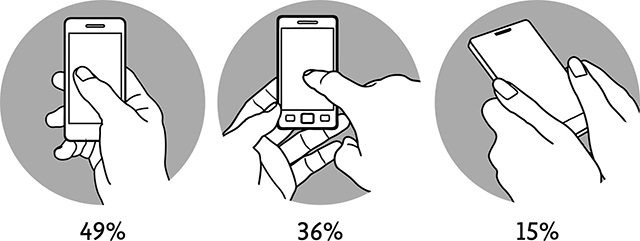
\includegraphics[width=\textwidth]{images/MobileWeb-Fitts}	
						\caption[Mobile Web - Impugnature e utilizzo] {Mobile Web - Tipi di impugnatura e percentuale di utilizzo}
						\label{fig:MobileWeb-Fitts}
					\end{figure}
					
					Come si vede dalla figura ~\ref{fig:MobileWeb-Fitts}, l'uso del pollice è preferito (75\%) e questo garantisce una \textbf{pessima precisione}. Ci sono poi delle zone di \textbf{bassa usabilità} perché raggiungibili solo allungando la mano, nel caso dei tablet peggio ancora, per questo i controlli dovrebbero essere sempre nella parte inferiore (come i controlli standard degli smartphone). Bisogna poi tenere conto che la forma dello schermo può cambiare da normale a landscape. La migliore interfaccia quindi deve tenere conto di tutti i casi e lasciare la possibilità all'utente di cambiare interfaccia.
					\subparagraph{Zone magiche}
						Riguardo le così definite \emph{zone magiche} su mobile non disponiamo di nessuna finestra. I \emph{fan menu} funzionano molto bene meno invece i \emph{pie menu} perché le dita coprono parti di schermo e quindi anche pulsanti.
					

%\include{sezioni/}

%\include{sezioni/}

%\include{sezioni/}

%\include{sezioni/}

%\include{sezioni/}

%\include{sezioni/}

%\include{sezioni/}


\end{document}	